\newcommand*{\TeXturedVERSION}{1.5.0} %% TeXtured 2025-08-06
%%%%%%%%%%%%%%%%%%%%%%%%%%%%%%%%%%%%%%%%%%%%%%%%%%%%%%%%%%%%%%%%%%%%%%%
%% NOTE: If you find any issues or have any suggestions, please open %%
%%       an Issue on GitHub: https://github.com/jdujava/TeXtured     %%
%%%%%%%%%%%%%%%%%%%%%%%%%%%%%%%%%%%%%%%%%%%%%%%%%%%%%%%%%%%%%%%%%%%%%%%

%% Enable built-in LaTeX support for PDF/A compliance (must be before `\documentclass`)
\DocumentMetadata{lang=en, pdfversion=1.7, pdfstandard=A-2u}
\input{preamble/pdfA-compliance/glyphtounicode}

%% NOTE: Choose the desirable page layout version (electronic vs print)
\documentclass[10pt,a4paper]{report}                      % single-side (electronic)
% \documentclass[12pt,a4paper,openright,twoside]{report}  % two-sided (for printing)

%% Set some toggle flags to control some of the document properties
\input{preamble/toggles}
% \FANCYfalse % disable some of the more fancy stylistic choices
%% NOTE: Comment out the following lines for the final version
%\WIPtrue            % THIS IS A WORK-IN-PROGRESS VERSION
% \EXTRAMARGINtrue  % add extra right margin in WIP version (for notes/corrections)
% \LINKBOXESfalse   % disable reference/link boxes for faster compilations
%\CENSORtrue         % THIS IS A CENSORED VERSION

%% Preamble - data, packages, macros, and more
\input{preamble/main}

%% Only uncommented files are included (faster compilation)
%% NOTE: If no files are uncommented, all files are included
\includeonlysmart{
    frontmatter/title,
    % frontmatter/declaration,
    % frontmatter/dedication,
    frontmatter/information,
    chapters/Chap1_design,
    chapters/Chap2_sync,
    chapters/Chap3_channel,
    chapters/chap5_transmission,
    chapters/Chap6_coding,
    %chapters/code,
    %chapters/Test,
    %chapters/Introduction,
    %chapters/QuickSummary,
    %chapters/Notation,
    %chapters/Design,
    %chapters/Usage,
    %chapters/Features,
    %chapters/Tips,
    %chapters/Summary,
    %chapters/Appendix,
    chapters/Appendix1,
}

\begin{document}

\frontmatter
\include{frontmatter/title}
% \include{frontmatter/declaration}
% \include{frontmatter/dedication}
% \include{frontmatter/information}

\contentsandlists

%\chapternotnumbered{Introduction} \label{ch:Introduction}

\vspace{2ex}

Orthogonal Frequency Division Multiplexing (OFDM) is a widely adopted transmission technique
for broadband communication over frequency-selective channels. By dividing a wideband
channel into a set of narrowband orthogonal subcarriers, OFDM effectively mitigates
Inter-Symbol Interference (ISI) and enables simpler equalization in the frequency
domain.

In this project, an acoustic OFDM communication system is designed, implemented, and
experimentally validated. Acoustic channels are particularly challenging due to severe
multipath propagation, long delay spreads, Doppler effects, and hardware-induced
imperfections. These impairments make synchronization, channel estimation, and phase
tracking critical components of the receiver design.

The objective of this work is threefold. First, a complete OFDM transceiver is implemented
in Matlab, including synchronization, channel estimation, equalization, and decoding.
Second, the system performance is evaluated across a set of emulated channels exhibiting
distinct impairments such as phase rotation, delay spread, band rejection, and multi-path
fading. Finally, the system is validated in a real acoustic environment through the
transmission of an image data, using the provided microphone and speakers.

Special attention is given to practical receiver algorithms, including Least Squares (LS)
and windowed LMMSE channel estimation, pilot-based phase tracking, and concatenated
Forward Error Correction (FEC). Performance is assessed using metrics such as Bit Error
Rate (BER), spectral efficiency, and channel impulse response characteristics.
\section*{Quick Summary}

This report presents the design, implementation, and validation of an acoustic OFDM communication system optimized for reverberant environments.

\Cref{ch:design} describes the complete transceiver architecture, including the OFDM frame structure, synchronization preamble, and pilot-assisted transmission.

\Cref{ch:sync} details the receiver synchronization algorithms, including normalized cross-correlation for packet detection, two-stage Carrier Frequency Offset (CFO) estimation, and pilot-based phase tracking to compensate for residual phase drift.

\Cref{ch:channel} evaluates the performance of Least Squares (LS) and windowed LMMSE channel estimation techniques across five distinct channel models, highlighting their strengths and limitations in the presence of noise, delay spread, and frequency-selective fading.

\Cref{ch:performance} analyzes the spectral efficiency of the implemented system and discusses the impact of modulation order, cyclic prefix length, training overhead, and payload size.

\Cref{ch:transmission} presents the results of a real acoustic image transmission experiment conducted in the Rolex Learning Center (RLC), demonstrating the system’s robustness to severe multipath propagation.

Finally, \Cref{ch:coding} evaluates the impact of concatenated channel coding on Bit Error Rate (BER) performance and discusses the associated trade-offs between robustness and throughput.

\Cref{ch:appendix_visual} provides extensive visual documentation of channel responses, equalized constellations, and experimental results.

\begin{Note}
    For detailed instructions on how to execute the simulations or manipulate the project files, please refer to the \textbf{Code Organization} section in \Cref{organization}.
\end{Note}
%\include{chapters/Notation}

\mainmatter
%\setcounter{chapter}{13} % "N" (14th letter, but latex first increments -> 14-1=13)
\chapter{Design Description \& Frame Construction } \label{ch:design}

The implemented architecture establishes a complete \textsf{OFDM} transceiver operating in baseband \autocite{Cimini1985}. To mimic a realistic transmission environment, the system simulates passband transmission through digital upconversion and downconversion steps. The system is logically divided into two primary processing blocks: the transmission chain and the reception chain.

\section{Transmission Chain}%
\label{sec:Transmission Chain}
\fileTeXtured{custom\_function/transmit/transmitter.m}

The transmission process is encapsulated within the \custommacro{transmitter} function. It orchestrates the transformation of raw binary data into a continuous time-domain waveform ready for the channel.

\begin{figure}[h]
    \fcapside[\FBwidth]{%
        \captionsetup{parskip = .5\baselineskip plus 1pt}%
        \caption[Time and Frequency Domain Representation of TX Symbols]{%
            Transmission Chain block diagram
        }%
        \label{fig:4}%
    }{%
        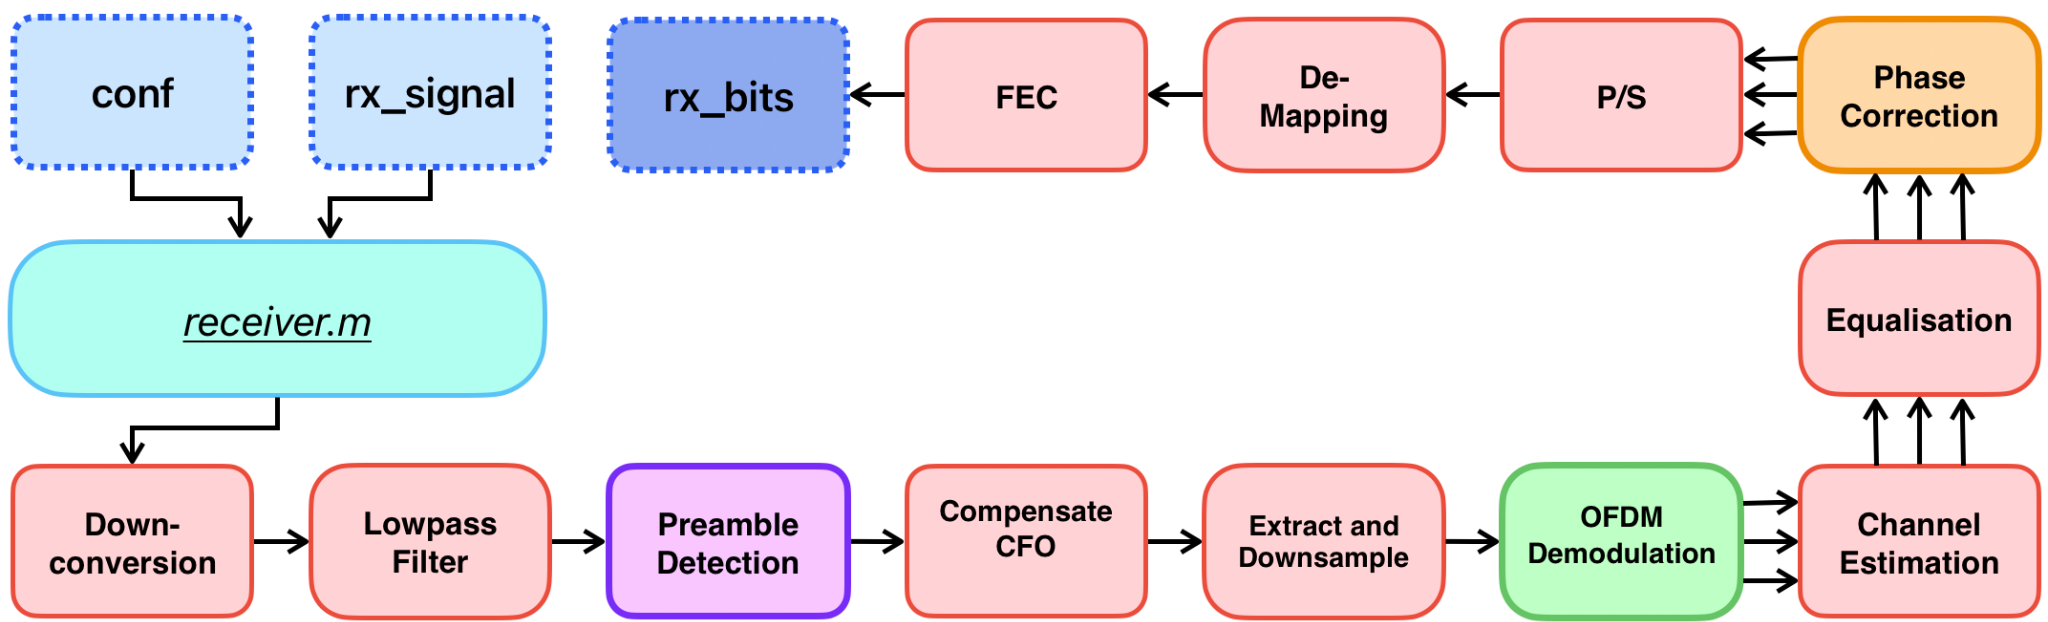
\includegraphics[width=0.80\textwidth]{figures/chap1_design/4.png}
    }
\end{figure}

\subsection{Payload Management and Concatenated FEC}%
\label{sub:Payload FEC}

The process begins with the generation or reception of the payload bits. All system parameters are centralized in \path{configurations.m}.
\begin{itemize}
    \item \textbf{Concatenated Coding:} If the Forward Error Correction (\textsf{FEC}) is enabled (via \path{conf.coding.use_fec}), the system employs a robust concatenated coding scheme implemented in \custommacro{channel\_encoder}. This architecture, along with its impact on overall link reliability, is analyzed in detail in \Cref{ch:performance}.
    
    \item \textbf{Symbol Mapping:} The encoded bit stream is mapped to complex symbols belonging to a configurable constellation (e.g., \textsf{QPSK}, \textsf{16-QAM}) defined in \path{conf.modulation}.
\end{itemize}

\begin{figure}[h]
    \fcapside[\FBwidth]{%
        \captionsetup{parskip = .5\baselineskip plus 1pt}%
        \caption[Time and Frequency Domain Representation of TX Symbols]{%
            OFDM Frame construction.
        }%
        \label{fig:4}%
    }{%
        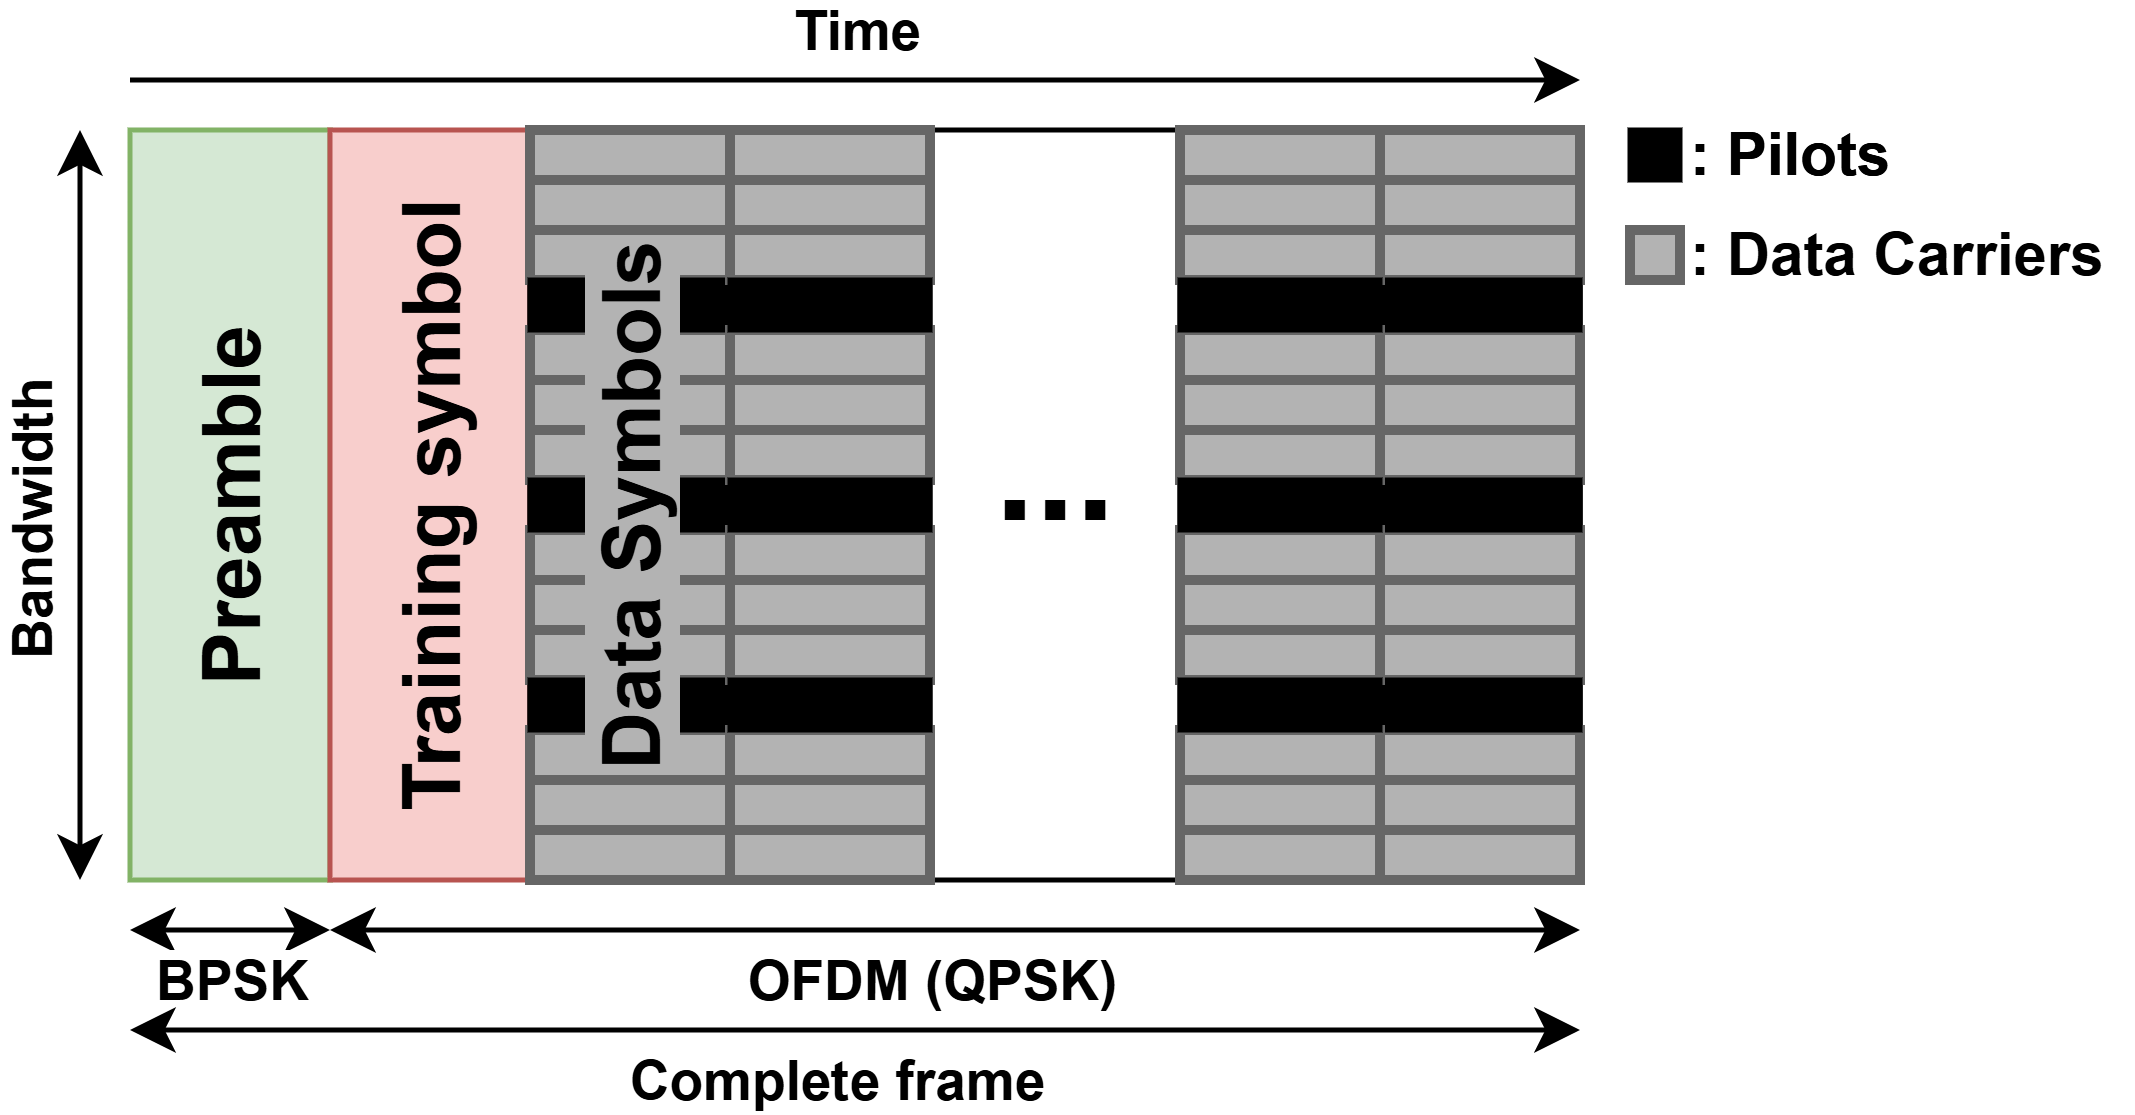
\includegraphics[width=0.70\textwidth]{figures/DrawIoSchematics/FrameStructure.png}
    }
\end{figure}

\subsection{OFDM Frame Construction}%
\label{sub:OFDM Frame Construction}
\fileTeXtured{.../ofdm\_tx\_frame\_with\_pilots.m}

The core signal construction is handled by the \custommacro{ofdm\_tx\_frame\_with\_pilots} function. This stage transforms the serial symbol stream into parallel frequency subcarriers:
\begin{enumerate}
    \item \textbf{Frequency Organization:} Data symbols are mapped onto the active subcarriers defined by the \path{conf.ofdm.psdMask}.
    \item \textbf{Training Symbol Insertion:} A dedicated \textbf{Training Symbol} (known to the receiver) is inserted as the very first OFDM symbol of the frame. This is strictly used for Channel Frequency Response (CFR) estimation and is distinct from the synchronization preamble.
    \item \textbf{Pilot Insertion:} Known pilot symbols are inserted at specific indices (defined in \path{conf.ofdm.pilotIndices}) within the data symbols. These pilots are crucial for tracking phase rotation caused by residual frequency offsets at the receiver.
    \item \textbf{IFFT \& Cyclic Prefix:} The frequency domain blocks are transformed into the time domain using the Inverse Fast Fourier Transform (\macro{ifft}). A Cyclic Prefix (CP) is appended to the beginning of each symbol to mitigate \emph{Inter-Symbol Interference} (ISI).
\end{enumerate}

\subsection{Finalization and Upconversion}%
\label{sub:Upconversion}

Following the OFDM modulation, the signal undergoes several conditioning steps in \custommacro{transmitter}:
\begin{enumerate}
    \item \textbf{Upsampling:} The OFDM signal is upsampled from the baseband bandwidth \autocite{Proakis2007} to the system sampling rate $f_s$ using \custommacro{ofdm\_tx\_resampling}.
    \item \textbf{Preamble Prepending:} To aid synchronization, a separate \textbf{Preamble sequence} (generated via LFSR) is prepended to the frame. Unlike the OFDM data, this preamble is a single-carrier sequence, upsampled and filtered with a Root-Raised Cosine (\textsf{RRC}) pulse to ensure good correlation properties.
    \item \textbf{Upconversion:} Finally, the signal is digitally upconverted to the carrier frequency $f_c$ by multiplying with a complex exponential $e^{j 2 \pi f_c t}$.
\end{enumerate}


\section{Reception Chain}%
\label{sec:Reception Chain}
\fileTeXtured{custom\_function/receive/receiver.m}

The receiver performs the inverse operations to recover the information from the noisy, distorted signal received from the channel.

\begin{figure}[h]
    \fcapside[\FBwidth]{%
        \captionsetup{parskip = .5\baselineskip plus 1pt}%
        \caption[Time and Frequency Domain Representation of TX Symbols]{%
            Reception chain block diagram.
        }%
        \label{fig:1}%
    }{%
        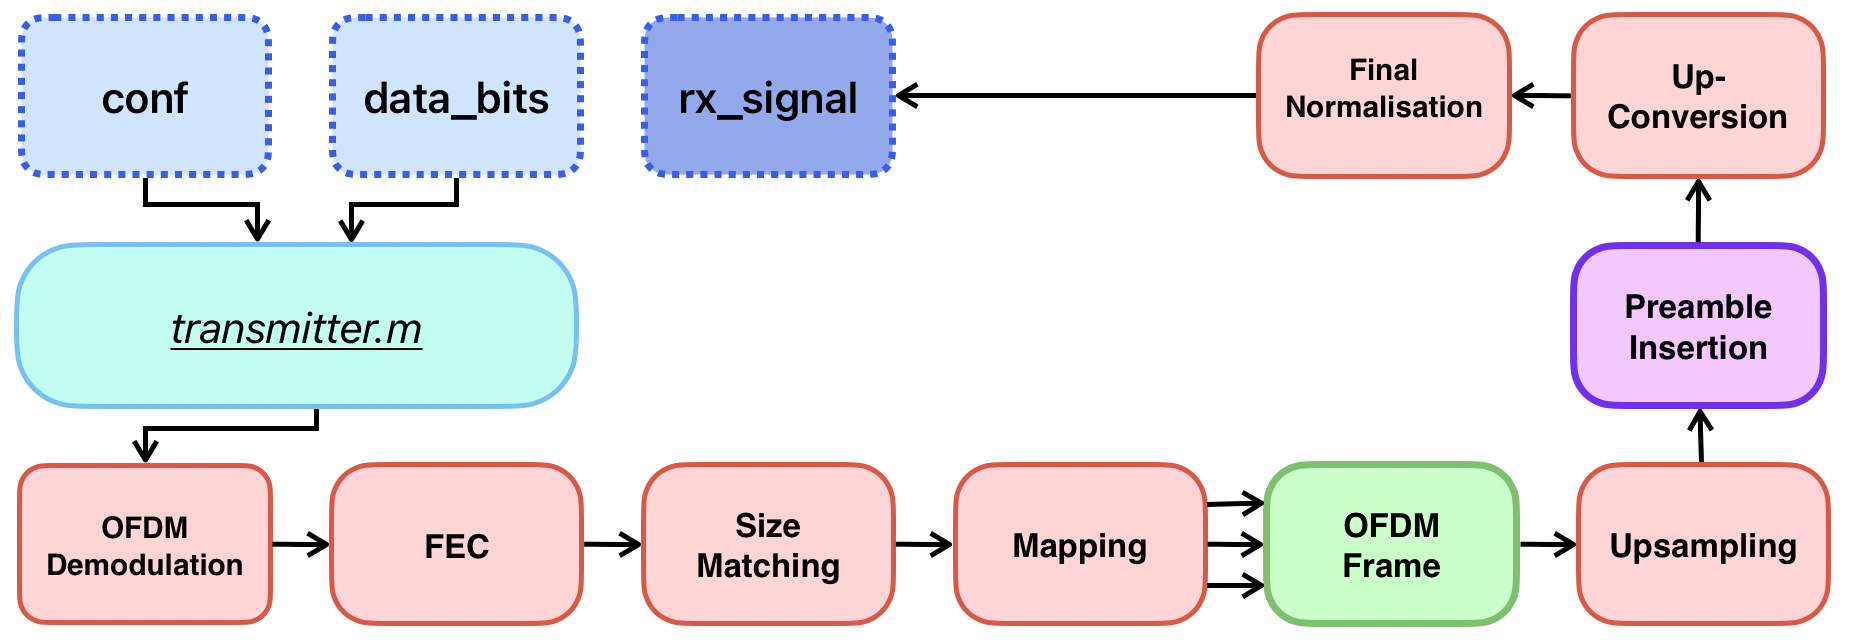
\includegraphics[width=0.80\textwidth]{figures/chap1_design/5.png}
    }
\end{figure}

\subsection{Downconversion and Filtering}%
\label{sub:Downconversion}

The received signal is first digitally downconverted from $f_c$ back to baseband. Immediately following the mixing, a low-pass filter is applied via \custommacro{ofdmlowpass} to remove double-frequency terms and out-of-band noise.

\subsection{Synchronization}%
\label{sub:Synchronization}
\fileTeXtured{custom\_function/receive/estimateTauAndCFO.m}

Before demodulation can occur, the receiver must synchronize in both time and frequency. This will be discussed in \Cref{ch:sync}.

\subsection{Channel Estimation and LMMSE Refinement}%
\label{sub:ChannelEst}
\fileTeXtured{.../receive/ChannelMetrics.m}

Once synchronized, the signal is resampled and the Cyclic Prefix is removed. The system then performs advanced channel estimation:
\begin{enumerate}
    \item \textbf{LS Estimation:} A Least Squares (LS) estimate is computed in \custommacro{channel\_estLS} by dividing the received \textbf{Training Symbol} (the first symbol of the frame) by the transmitted reference.
    \item \textbf{Asymmetric LMMSE Smoothing:} The LS estimate is refined using a practical \textsf{LMMSE} approach in \custommacro{ChannelMetrics}. This function:
    \begin{itemize}
        \item Transforms the LS estimate to the time domain (CIR).
        \item Centers the energy peak using circular shifts.
        \item Applies an \textbf{asymmetric window} defined by \path{conf.ch.back} (pre-cursors) and \path{conf.ch.length} (post-cursors) to filter out noise while preserving the multipath taps.
        \item Transforms back to the frequency domain to obtain the cleaned $\hat{H}_{\text{LMMSE}}$.
    \end{itemize}
\end{enumerate}
The data symbols are then equalized using the cleaned coefficients. Finally, residual phase rotations are tracked and corrected symbol-by-symbol using the pilot subcarriers via \custommacro{correctOFDMSymbolRotation}.

\begin{figure}[h]
    \fcapside[\FBwidth]{%
        \captionsetup{parskip = .5\baselineskip plus 1pt}%
        \caption[Time and Frequency Domain Representation of TX Symbols]{%
            Example of low resolution transmitted image.
        }%
        \label{fig:1}%
    }{%
        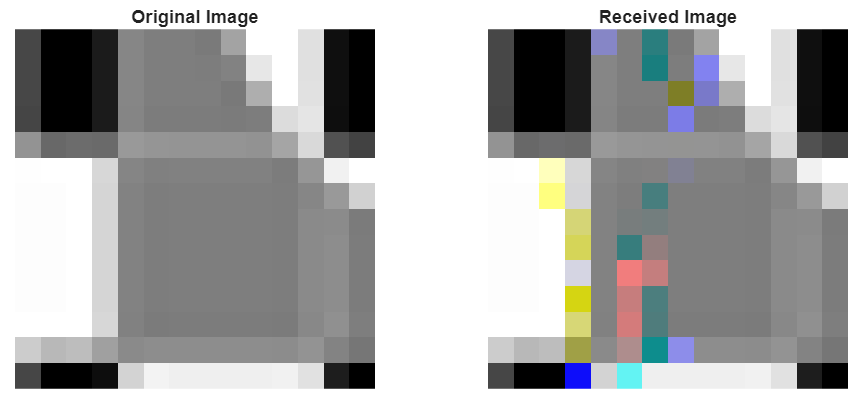
\includegraphics[width=0.80\textwidth]{figures/chap1_design/3.png}
    }
\end{figure}

\subsection{Decoding}%
\label{sub:Decoding}
\fileTeXtured{custom\_function/receive/channel\_decoder.m}

The equalized complex symbols are demapped into bits. If \textsf{FEC} is enabled, the bits are processed by the concatenated decoder (see \Cref{ch:coding}):
\begin{enumerate}
    \item \textbf{Viterbi Decoder:} The inner decoding step uses the Viterbi algorithm (hard decision) with a traceback depth defined in \path{conf.coding.traceBackDepth} to correct errors from the channel.
    \item \textbf{Reed-Solomon Decoder:} The outer decoding step processes the Viterbi output to correct any remaining block errors, providing the final estimated payload.
\end{enumerate}


\newpage
\section{Code Organization} \label{organization}
\begin{figure}[!ht]
    \fcapside[\FBwidth]{%
        \captionsetup{parskip = .5\baselineskip plus 1pt}%
        \caption[Project File Structure and Usage]{%
            \textbf{Structure and Usage Guide.}
            
            The project code is organized into a root directory containing the execution scripts and configuration, with modular functions separated by purpose.
            
            \textbf{Execution Flow:} The main entry point is \path{main.m}, which runs the complete image transmission experiment. It loads the image from \path{img/}, encodes it, transmits it (via audio or emulator), and reconstructs the received result. For performance analysis, \path{dbg_channelPlot.m} generates BER curves vs SNR, while \path{dbg_equalizationComp.m} compares different equalizer settings.

            \path{main_singleChannel al.m} tests OFDM transmission performance on a single channel by sending random payloads through the emulated channel at a fixed SNR. It computes Bit Error Rate (BER), Packet Error Rate (PER), and goodput over multiple packets.
            
            \textbf{Configuration:} All system parameters are centralized in \path{configurations.m}. This includes the OFDM setup (512 subcarriers, CP length), signal parameters ($f_s=48$kHz), and channel model selection. Modify this file to change the experiment conditions.
            
            \textbf{Core Modules:} The \path{custom_function/} directory houses the user-implemented logic. It is split into \path{transmit/} (encoder, frame builder) and \path{receive/} (synchronization, channel estimation, decoding). Helper scripts like \path{preamble_generate.m} reside in the root of this folder. The \path{provided_function/} directory contains the pre-compiled channel emulator and standard filters provided for the course.
        }%
        \label{fig:project-structure}%
    }{%
        \begin{tikzpicture}[dirtree]
            \node[directory] {OFDM Project/}
            child { node {configurations.m}}
            child { node {main.m}}
            child { node {main\_singleChannel.m}}
            child { node {dbg\_channelPlot.m}}
            child { node {dbg\_equalizationComp.m}}
            child { node[directory] {custom\_function/}
                child { node {preamble\_generate.m}}
                child { node {tfplotReImPhase.m}}
                child { node[directory] {receive/}
                    child { node {receiver.m}}
                    child { node {estimateTauAndCFO.m}}
                    child { node {ChannelMetrics.m}}
                    child { node {channel\_estLS.m}}
                    child { node {channel\_decoder.m}}
                    child { node {correctOFDMSymbolRotation.m}}
                    child { node {ofdm\_rx\_frame.m}}
                }
                child [missing] {} child [missing] {} child [missing] {} child [missing] {} child [missing] {} child [missing] {} child [missing] {} 
                child { node[directory] {transmit/}
                    child { node {transmitter.m}}
                    child { node {ofdm\_tx\_frame\_with\_pilots.m}}
                    child { node {channel\_encoder.m}}
                }
            }
            child [missing] {} child [missing] {} child [missing] {} child [missing] {} child [missing] {} child [missing] {} child [missing] {} child [missing] {} child [missing] {} child [missing] {} child [missing] {} child [missing] {}
            child [missing] {} child [missing] {}
            child { node[directory] {img/}
                child { node {test-image.bmp}}
                child { node {received\_image.bmp}}
            }
            child [missing] {}
            child { node[directory] {provided\_function/}
                child { node {channel\_emulator.p}}
                child { node {ofdmlowpass.m}}
                child { node {rrc.m}}
                child { node {ofdm\_rx\_resampling.m}}
                child { node {ofdm\_tx\_resampling.m}}
            }
            ;
        \end{tikzpicture}%
    }
\end{figure}

%\setcounter{chapter}{13} % "N" (14th letter, but latex first increments -> 14-1=13)
\chapter{Synchronization Method} \label{ch:sync}


Reliable OFDM communication relies heavily on maintaining orthogonality between subcarriers.
In a real acoustic environment, hardware imperfections and channel propagation introduce time delays and frequency offsets that destroy this orthogonality.
Consequently, before any demodulation or channel estimation can occur, the receiver must perform a rigorous synchronization process.
This chapter details the implemented techniques for packet detection, frequency correction, and phase tracking \autocite{Schmidl1997}.

\section{Time Synchronization (Packet Detection)} \label{sec:TimeSync}

The first stage of the receiver pipeline is to identify the precise start of the data packet within the incoming stream of samples.
This is achieved using a known \textbf{Preamble} sequence prepended to the frame.
The function \texttt{estimateTauAndCFO} implements a normalized cross-correlation algorithm to locate this sequence.

Mathematically, the timing metric $M(d)$ at delay $d$ is computed as:
\begin{equation}
    M(d) = \frac{|\sum_{n=0}^{L-1} r^*[d+n] p[n]|^2}{\sum_{n=0}^{L-1} |r[d+n]|^2},
\end{equation}
where $r[n]$ is the received signal, $p[n]$ is the known preamble, and $L$ is the preamble length.
Normalization by the received energy (the denominator) is crucial to ensure the thresholding mechanism remains robust against varying volume levels in the acoustic channel.

As shown in \Cref{fig:correlation_metric}, the algorithm searches for a peak in $M(d)$ that exceeds a predefined threshold (\texttt{conf.preamble.thr}).
Once the peak is detected, the index is refined to pinpoint the exact sample marking the end of the preamble and the beginning of the payload.

\begin{figure}[!ht]
    \fcapside[\FBwidth]{%
        \captionsetup{parskip = .5\baselineskip plus 1pt}%
        \caption[Frame Detection Metric]{%
            Signal magnitude (top) and normalized correlation metric (bottom) used for frame detection.
            The distinct peak in the correlation metric $M(d)$ identifies the precise synchronization point $\tau$ despite the noisy received amplitude.
        }%
        \label{fig:correlation_metric}%
    }{%
        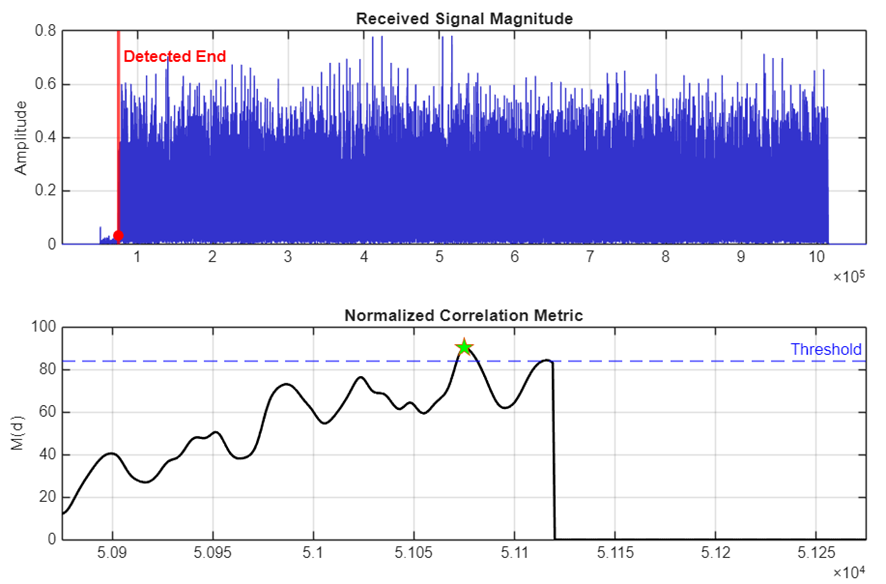
\includegraphics[width=0.60\textwidth]{figures/chap3_channel/c4_5.png}
    }
\end{figure}

\section{Frequency Synchronization (CFO Estimation)} \label{sec:FreqSync}

Oscillator mismatches between the transmitter (laptop) and receiver (microphone) introduce a Carrier Frequency Offset (CFO).
Left uncorrected, CFO causes a progressive phase rotation of the constellation symbols, leading to Inter-Carrier Interference (ICI).
The system mitigates this via a two-stage estimation process embedded in \texttt{estimateTauAndCFO}:

\begin{enumerate}
    \item \textbf{Coarse Estimation:} A grid search is performed over a range of potential frequency offsets (defined in \texttt{ofdmc.rangeCFO}). The system de-rotates the received preamble by each candidate frequency and computes the correlation. The frequency yielding the maximum response is selected as the coarse estimate.
    \item \textbf{Fine Estimation:} To achieve sub-grid precision, the system applies quadratic interpolation (parabolic fitting) around the coarse peak. This estimates the true maximum of the correlation function, providing a highly accurate CFO value.
\end{enumerate}

The entire received signal is then multiplied by $e^{-j2\pi \Delta f t}$ to compensate for the estimated offset $\Delta f$.

\section{Channel Estimation and Pilots} \label{sec:PilotsTraining}

Once synchronized, the receiver must compensate for the channel's spectral distortion.
The frame structure includes a dedicated \textbf{Training Symbol} located immediately after the preamble.
This symbol contains known values on all active subcarriers.
By comparing the received training symbol to the transmitted reference, the Least Squares (LS) estimator computes the initial Channel Frequency Response (CFR), as detailed in \Cref{ch:channel}.

\subsection{Phase Tracking with Pilots}
While the Training Symbol provides a snapshot of the channel at the beginning of the frame, residual CFO or slow channel variations can cause the phase to drift over the duration of the packet.
To counter this, \textbf{Pilot Symbols} are inserted into specific subcarriers (e.g., indices defined in \texttt{ofdmc.pilotIndices}) of every OFDM data symbol.

The function \texttt{correctOFDMSymbolRotation} extracts these pilots after equalization.
It computes the residual phase rotation $\theta_m$ for the $m$-th OFDM symbol by averaging the phase difference between the received pilots and the known transmitted pilots.
This per-symbol correction ensures the constellation remains stable throughout the transmission, preventing the "spinning" effect common in uncorrected OFDM systems.

\section{Cyclic Prefix (CP)} \label{sec:CP}

To combat multipath propagation—clearly visible in the taps of \Cref{fig:trans_cir_pdp} (Appendix)—a \textbf{Cyclic Prefix} is prepended to every OFDM symbol.
The CP acts as a guard interval, absorbing the Inter-Symbol Interference (ISI) caused by delayed echoes.
Crucially, it converts the linear convolution of the channel into a circular convolution, which is the mathematical prerequisite (\autocite{NeePrasad2000}) for simple single-tap equalization in the frequency domain.

As discussed in \Cref{ch:channel}, the length of the CP determines the maximum delay spread the system can tolerate.
While a conservative length (e.g., 256 samples) ensures robustness in reverberant rooms (Channel 5), it reduces spectral efficiency.
Adaptive CP scaling remains a viable optimization for benign channels (Channels 1 and 2). This will also be analyzed in detail in \Cref{ch:transmission} for each channel.
%\setcounter{chapter}{13} % "N" (14th letter, but latex first increments -> 14-1=13)
\chapter{Channel Estimation} \label{ch:channel}

In this chapter, we present a detailed analysis of the five proposed communication channels.
Metrics such as frequency response, $\gamma_{\text{ISI}}$, Power Delay Profile (PDP), and Bit Error Rate (BER) were utilized to characterize and compare their performance.
The varying nature of these channels introduces distinct impairments that complicate reliable transmission.

\section{Quantification of ISI}%
\label{sec:ISI Characterization}
\dirTeXtured{chapters/ISI/}

The phenomenon of Intersymbol Interference (ISI) arises from the time dispersion $T_p$ of the physical channel, which is formally defined by the interval $t_{inf} \le t \le t_{sup}$ where the impulse response $p(t)$ remains non-zero. As discussed in \textcite{ComunicacionesDigitales2012}, the discrete equivalent model $p[n]$ captures the interference between adjacent symbols. By normalizing the observation by the cursor $p[d]$, we decompose the signal at the decider input into three fundamental components:
\begin{figure}[!ht]
    \fcapside[\FBwidth]{%
        \captionsetup{parskip = .5\baselineskip plus 1pt}%
        \caption[Time Dispersion and Discrete Mapping]{%
            Impulse response $p(t)$ illustrating the relation between $T_p$ and the sampled coefficients $p[n]$ \autocite{Artes2012}.
        }%
        \label{fig:isi-dispersion}%
    }{%
        
\includegraphics[width=0.4\textwidth]{figures/chap3_channel/1.png}
    }
\end{figure}
\begin{equation} \label{eq:ISI_decomposition}
    \frac{q[n]}{p[d]} = A[n-d] + \sum_{k \neq d} \frac{p[k]}{p[d]} A[n-k] + \frac{z[n]}{p[d]} \eqend
\end{equation}
To evaluate the system's performance, we analyze the worst-case error bound using the triangle inequality:
\begin{align}
    \left| \frac{q[n]}{p[d]} - A[n-d] \right| &= \left| \sum_{k \neq d} \frac{p[k]}{p[d]} A[n-k] + \frac{z[n]}{p[d]} \right| \nonumber \\
    &\le |A|_{\text{max}} \underbrace{\sum_{k \neq d} \frac{|p[k]|}{|p[d]|}}_{D_{\text{peak}}} + \frac{|z[n]|}{|p[d]|} \label{eq:ISI_bound_derivation}
\end{align}
The relationship between the \emph{peak distortion} $D_{\text{peak}}$ and the constellation's \emph{robustness factor} $\eta$ determines the total ISI level $\gamma_{\text{ISI}}$. These parameters are defined as:
\begin{equation} \label{eq:ISI_metrics}
    D_{\text{peak}} \doteq \sum_{k \neq d} \frac{|p[k]|}{|p[d]|} \eqcomma \qquad \eta \doteq \frac{d_{\text{min}}/2}{|A|_{\text{max}}} \eqcomma \qquad \gamma_{\text{ISI}} \doteq \frac{D_{\text{peak}}}{\eta} \eqend
\end{equation}
By substituting \eqref{eq:ISI_metrics} into the error bound \eqref{eq:ISI_bound_derivation}, we obtain the final condition for error-free transmission in noiseless scenarios ($z[n]=0$):
\begin{equation} \label{eq:final_ISI_bound}
    \left| \frac{q[n]}{p[d]} - A[n-d] \right| \le \gamma_{\text{ISI}} \left( \frac{d_{\text{min}}}{2} \right) + \frac{|z[n]|}{|p[d]|} \eqend
\end{equation}
\begin{remark}[Eye Diagram Closure]
    If $\gamma_{\text{ISI}} < 1$, the eye diagram remains open, meaning the distortion is smaller than the decision distance $d_{\text{min}}/2$. Conversely, when $\gamma_{\text{ISI}} > 1$, the interference alone causes errors, regardless of the Signal-to-Noise Ratio (SNR).
\end{remark}
\begin{Note}[Rate Dependency]
    The number of interfering samples $K = \lfloor T_p / T \rfloor$ increases as the transmission rate $R=1/T$ grows. Thus, a fixed dispersive channel may exhibit negligible ISI at low speeds but become unusable as $T$ decreases below $T_p$.
\end{Note}

\section{Methodology} \label{sec:Methodology}

To evaluate the channels, we employed a Least Squares (LS) estimation technique \autocite{Edfors1998}.
The LS algorithm derives the channel estimate from the training symbol located immediately after the preamble, representing a full OFDM symbol.
The channel frequency response, denoted as $\hat{H}[k]$, is obtained by dividing the received signal $Y[k]$ by the known pilot symbols $X[k]$ for each subcarrier $k$:
\begin{equation}
    \hat{H}_{\text{LS}}[k] = \frac{Y[k]}{X[k]}.
\end{equation}
When specific subcarriers are deactivated using a spectral mask, estimation is performed solely on the active frequencies.
By applying the Inverse Fast Fourier Transform (IFFT) to these frequency coefficients, we obtain the Channel Impulse Response (CIR).

\subsection{Practical MMSE Approximation} \label{sub:PracticalMMSE}

Observation of the CIR reveals that for most channels---particularly those exhibiting multipath propagation---the energy is concentrated in a finite duration.
The raw LS estimation, however, captures noise across the entire observation window, resulting in a \enquote{noisy} frequency response.
To mitigate this, we implemented a practical approximation of the Minimum Mean Square Error (MMSE) estimator.
This technique involves \enquote{windowing} the time-domain CIR: retaining the significant initial samples (taps) that represent the physical channel and zero-padding the rest.
Applying the FFT to this cleaned CIR yields a smoothed spectral estimate.
Mathematically, this approaches the theoretical MMSE solution and functions analogously to a low-order Moving Average process, significantly improving BER by rejecting noise outside the channel's delay spread.

\section{Channel 1: AWGN and Receiver Filtering} \label{sec:Channel1}

Channel 1 represents a classical Additive White Gaussian Noise (AWGN) scenario.
Ideally, an AWGN channel affects neither the phase nor the magnitude of the transmitted signal, implying that equalization might be unnecessary.
Examination of the impulse response confirms it approximates a delta function; however, the received signal is shaped by the receiver's front-end filter (typically an 8k band-pass filter).
Consequently, subcarriers at the band edges suffer varying degrees of attenuation compared to the center frequencies.

While LS equalization could invert this effect, it indiscriminately amplifies the noise.
The practical MMSE approach is superior here, as it models the filter's shape without enhancing the noise floor.
\Cref{fig:ch1_constellation_comparison} illustrates the resulting open eye pattern, confirming low Inter-Symbol Interference (ISI).

\begin{figure}[!ht]
    \centering
    \captionsetup{parskip = .5\baselineskip plus 1pt}
    \begin{tabular}{ccc}
        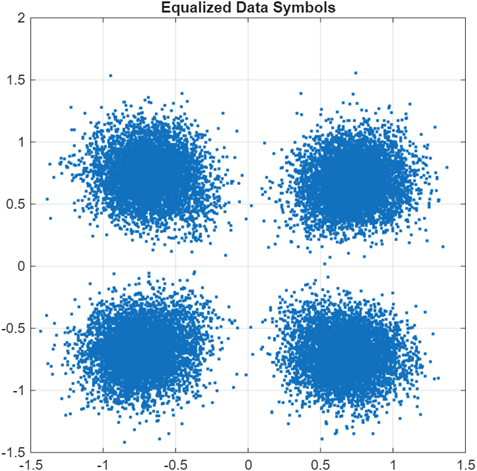
\includegraphics[width=0.3\textwidth]{figures/chap3_channel/c1_3.png} &
        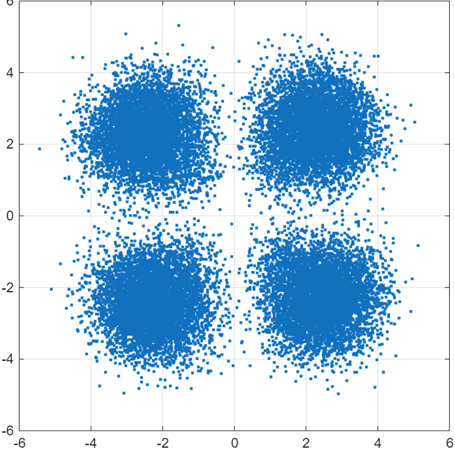
\includegraphics[width=0.3\textwidth]{figures/chap3_channel/c1_4.png} &
        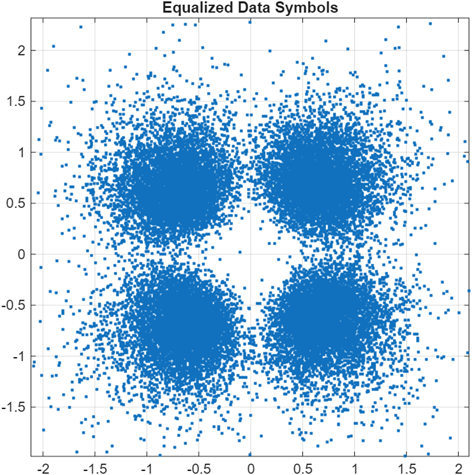
\includegraphics[width=0.3\textwidth]{figures/chap3_channel/c1_2.png} \\
        \small (a) MMSE Equalization & \small (b) LS Equalization & \small (c) No Equalization
    \end{tabular}
    \caption[Channel 1: Comparison of Equalization Techniques]{%
        Constellation comparison for Channel 1: (a) MMSE equalization provides optimal clustering; 
        (b) LS equalization shows higher noise sensitivity; 
        (c) Unequalized signal exhibiting an open eye pattern due to low ISI levels.
    }%
    \label{fig:ch1_constellation_comparison}%
\end{figure}

The impulse response and frequency magnitude are detailed in the appendix (see \Cref{fig:ch1_channel_estimation_summary}). The slight attenuation at the band edges is visible in the frequency response, which the MMSE estimator tracks smoothly.

\newpage

For Channel~1 (AWGN), the system achieves BER $<$ 1\% at about 3.5~dB SNR, both with and without FEC. As shown in Figure~\ref{fig:BERChannel1}, the coding gain from FEC becomes noticeable only at higher SNR values or for very low BER targets.

\begin{figure}[!ht]
    \fcapside[\FBwidth]{%
        \captionsetup{parskip = .5\baselineskip plus 1pt}%
        \caption[]{%
             Physical experimental setup showing the acoustic transmission environment.
        }%
        \label{fig:BERChannel1}%
    }{%
        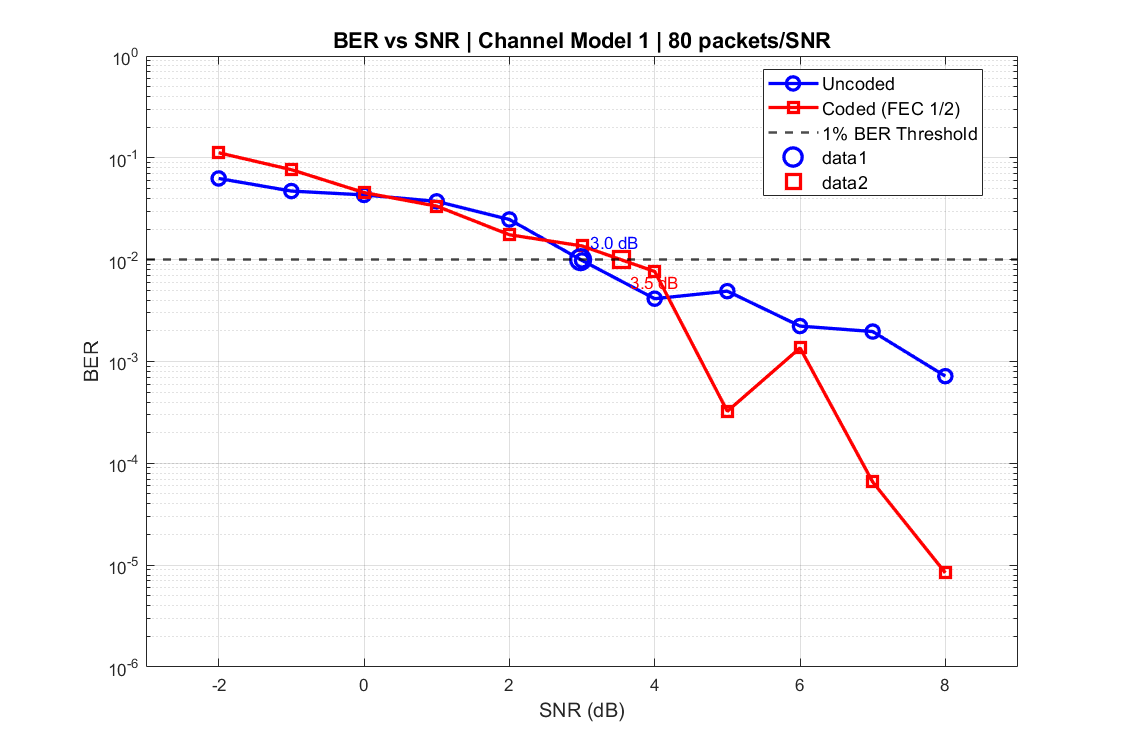
\includegraphics[width=0.70\textwidth]{figures/chap3_channel/BERChannel1.png}
    }
\end{figure}

\section{Channel 2: Phase Shift} \label{sec:Channel2}

Channel 2 shares the noise characteristics of Channel 1 but introduces a distinct phase shift.
Since the channel estimation is performed on a single training symbol at the start of the frame, time-varying phase drifts would only be visible if estimation were performed on a per-symbol basis.
However, in this static context, the constant phase rotation is evident.

Fortunately, the implemented synchronization system, which utilizes known QPSK pilots inserted into specific subcarriers of every data symbol, automatically corrects this phase offset.
Therefore, the performance and equalization strategies remain consistent with Channel 1. The effect of the equalization on the constellations is shown in \Cref{fig:ch2_constellations} in the appendix.

The channel estimation report (see \Cref{fig:ch2_report}) confirms a low ISI index, similar to the AWGN case.

\begin{figure}[!ht]
    \ffigbox[\FBwidth]{%
        \begin{tabular}{cc}
            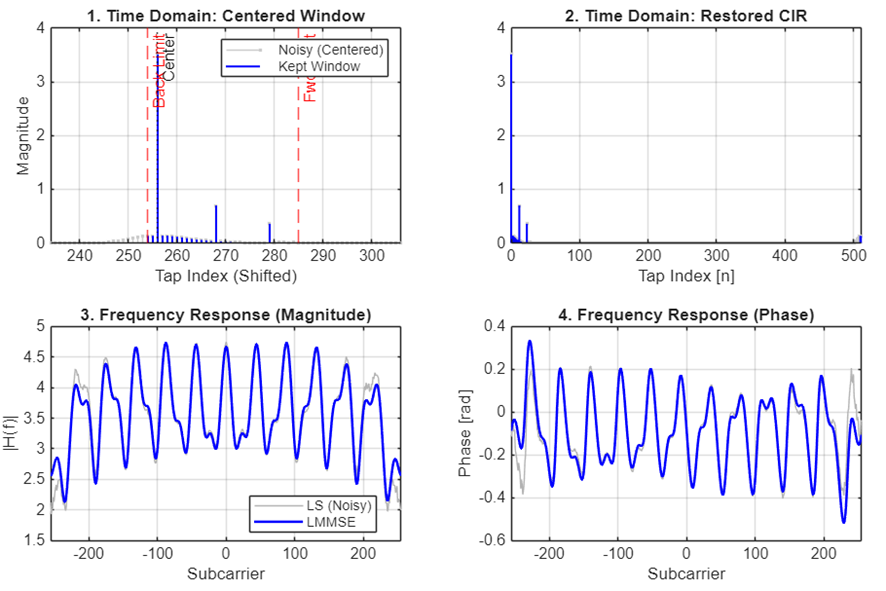
\includegraphics[width=0.67\textwidth]{figures/chap3_channel/c3_1.png} & 
            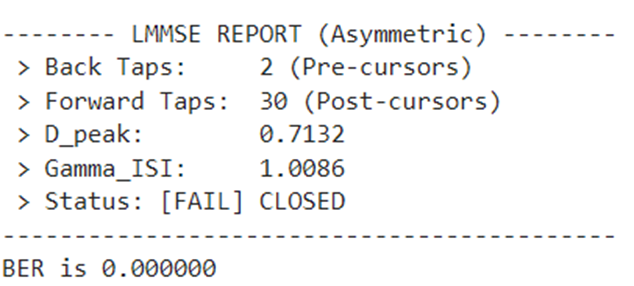
\includegraphics[width=0.27\textwidth]{figures/chap3_channel/c3_2.png} \\
        \end{tabular}
    }{%
        \caption[Channel Estimation and ISI Report]{%
            (Left) Time domain CIR windowing and Frequency Response analysis. 
            (Right) LMMSE numerical report with $\gamma_{\text{ISI}} = 1.0086$, confirming a closed eye status.
        }%
        \label{fig:channel_estimation_summary}%
    }
\end{figure}

\section{Channel 3: High Delay Spread} \label{sec:Channel3}

Channel 3 presents a unique challenge, visually resembling a \enquote{mandala} in the received signal constellation before equalization.
The frequency response exhibits rapid fluctuations in magnitude, characteristic of severe frequency-selective fading.
Contrary to the previous channels, the noise floor appears low, but the impulse response is exceptionally long, with significant peaks repeating approximately every 12 samples, as seen in the Power Delay Profile (PDP) in \Cref{fig:isi-dispersion}.

\begin{remark}[Equalization Strategy]
    Unlike the multipath channels discussed later, employing the windowed MMSE approximation here is detrimental.
    Truncating the long impulse response eliminates vital channel information spread across the delay line.
    Consequently, the LS estimator yields significantly better performance, producing highly clustered equalized symbols (see \Cref{fig:constellation_comparison}).
\end{remark}

\begin{figure}[!ht]
    \centering
    \captionsetup{parskip = .5\baselineskip plus 1pt}
    \begin{tabular}{ccc}
        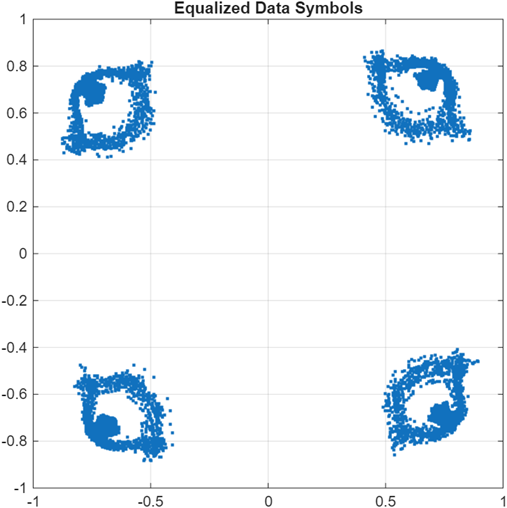
\includegraphics[width=0.3\textwidth]{figures/chap3_channel/c3_3.png} &
        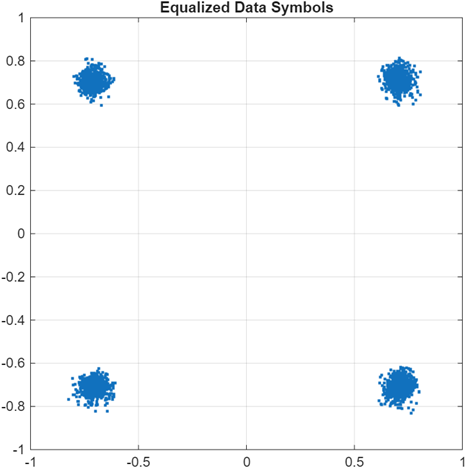
\includegraphics[width=0.3\textwidth]{figures/chap3_channel/c3_4.png} &
        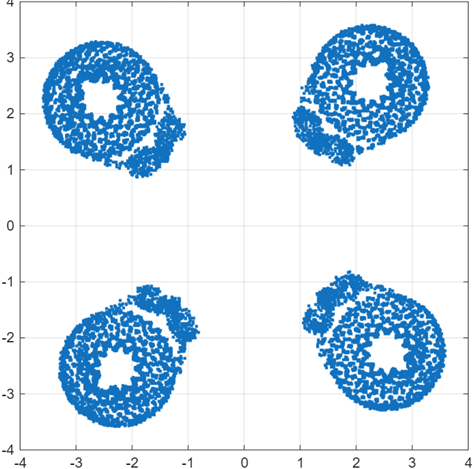
\includegraphics[width=0.3\textwidth]{figures/chap3_channel/c3_5.png} \\
        \small (a) MMSE Equalization & \small (b) LS Equalization & \small (c) No Equalization
    \end{tabular}
    \caption[Comparison of Equalization Techniques]{%
        Constellation comparison: (a) MMSE equalization provides optimal clustering; 
        (b) LS equalization shows higher noise sensitivity; 
        (c) Unequalized signal with a closed eye pattern due to severe ISI.
    }%
    \label{fig:constellation_comparison}%
\end{figure}

Regarding ISI, the numerical metric calculated yields $\gamma_{\text{ISI}} \approx 1.0086$, suggesting channel closure (see \Cref{fig:channel_estimation_summary}).
However, visual inspection of the constellation suggests a much lower effective ISI (approximately 0.5), with clearly separable symbols.
This discrepancy likely arises because the ISI metric is computed from the estimated channel response, which inevitably includes estimation noise, inflating the calculated interference.

\section{Channel 4: Band Rejection} \label{sec:Channel4}

Initial transmission over Channel 4 resulted in a scattered constellation resembling a chaotic cloud, yielding a BER of nearly 0.5.
Analysis of the frequency response reveals a deep spectral notch or band-rejection characteristic, where the magnitude of central subcarriers drops to near zero (see \Cref{fig:ch4_frequency_report}).
Inverting such a channel causes the equalizer to amplify noise infinitely at the nulls (singular matrix problem).

\begin{figure}[!ht]
    \fcapside[\FBwidth]{%
        \captionsetup{parskip = .5\baselineskip plus 1pt}%
        \caption[]{%
             Frequency response analysis revealing a significant band rejection.
        }%
        \label{fig:ch3_freqResp}%
    }{%
        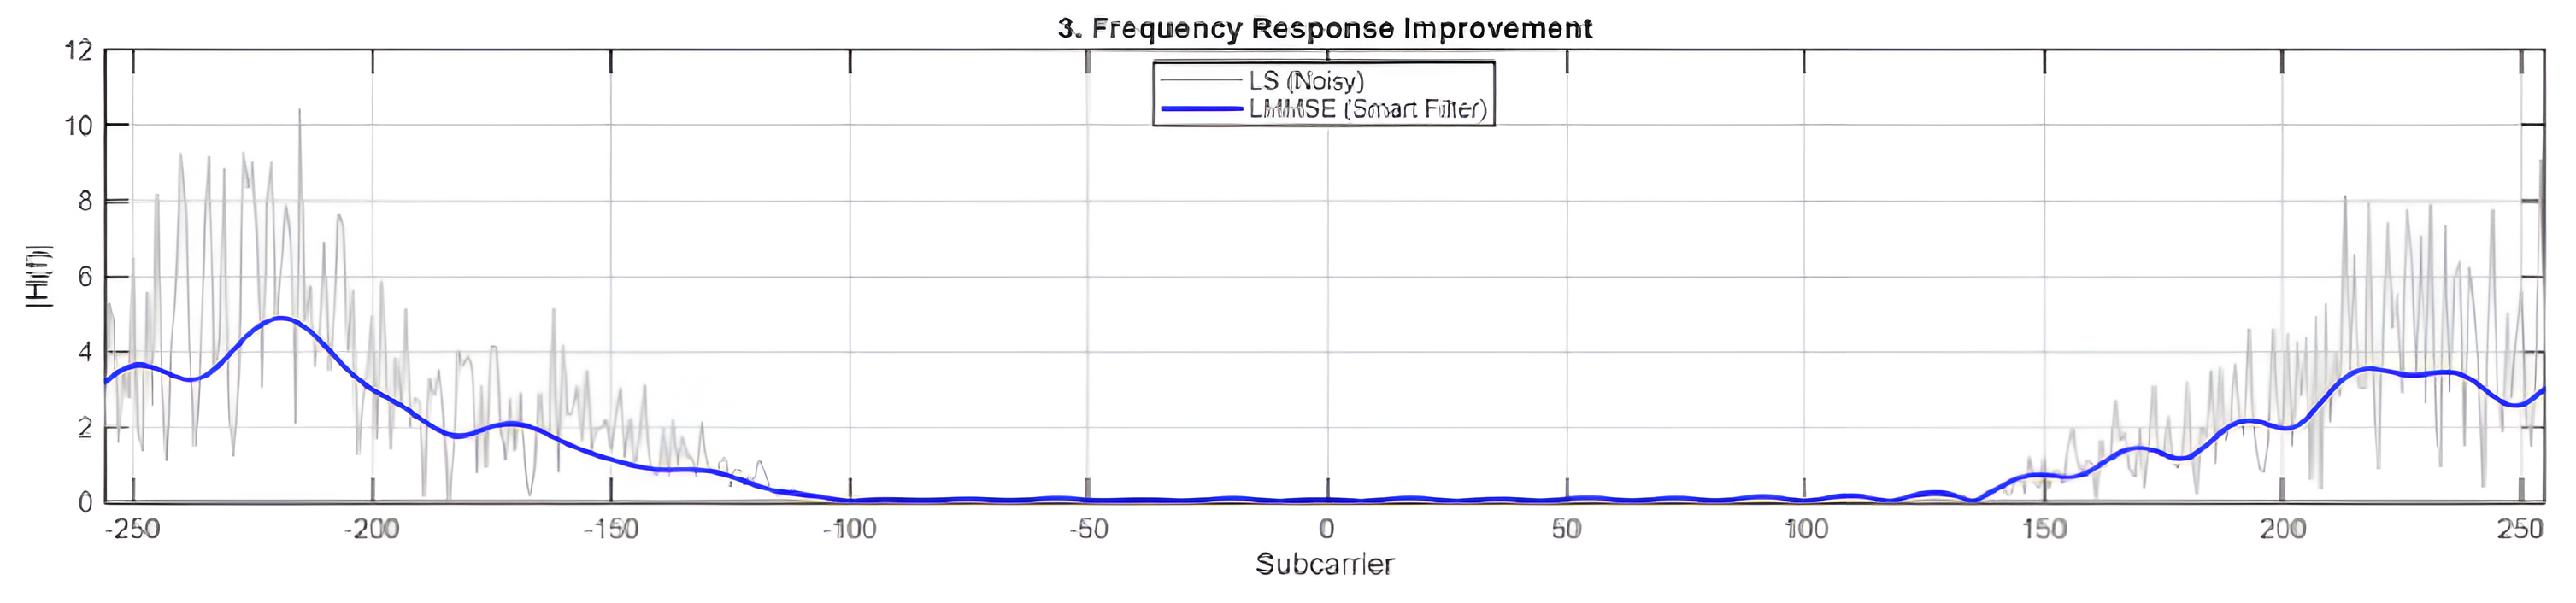
\includegraphics[width=0.70\textwidth]{figures/chap3_channel/c4_7.png}
    }
\end{figure}

To circumvent this, we adopted a sideband transmission strategy, deactivating the subcarriers within the rejection band.
While this necessitated increasing the frame duration to maintain data throughput, it successfully bypassed the deep fade.
As shown in \Cref{fig:ch4_constellations}, this strategy reduced the BER to \num{0.023107}.

\begin{figure}[!ht]
    \centering
    \captionsetup{parskip = .5\baselineskip plus 1pt}
    \begin{tabular}{cc}
        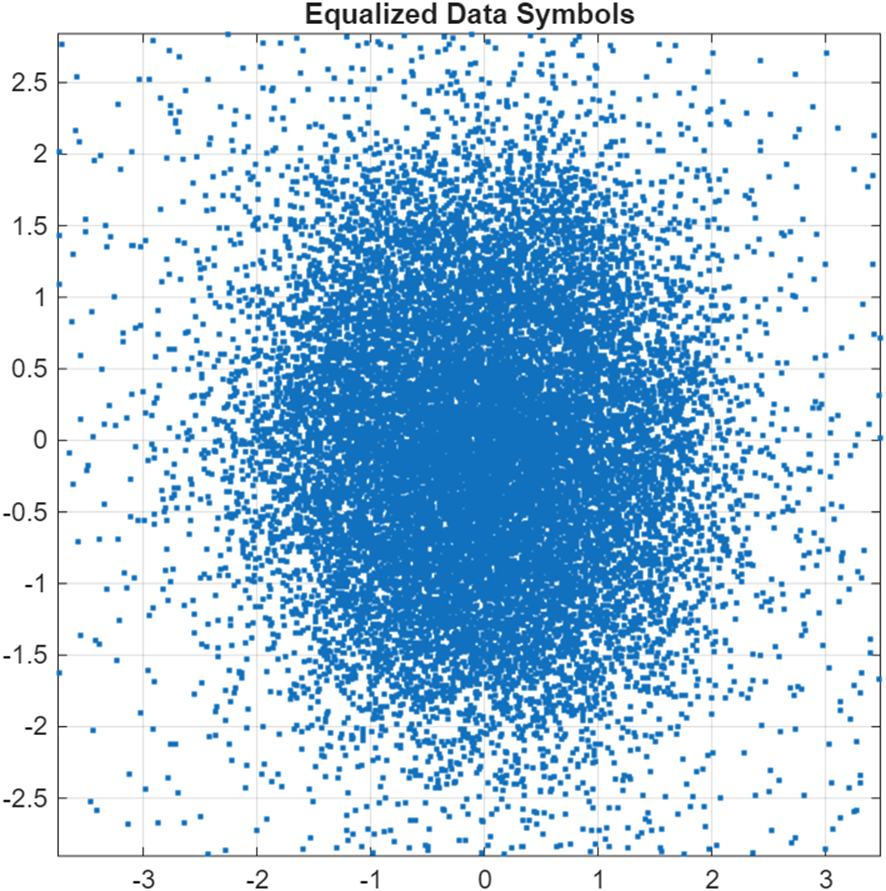
\includegraphics[width=0.45\textwidth]{figures/chap3_channel/c4_1.png} &
        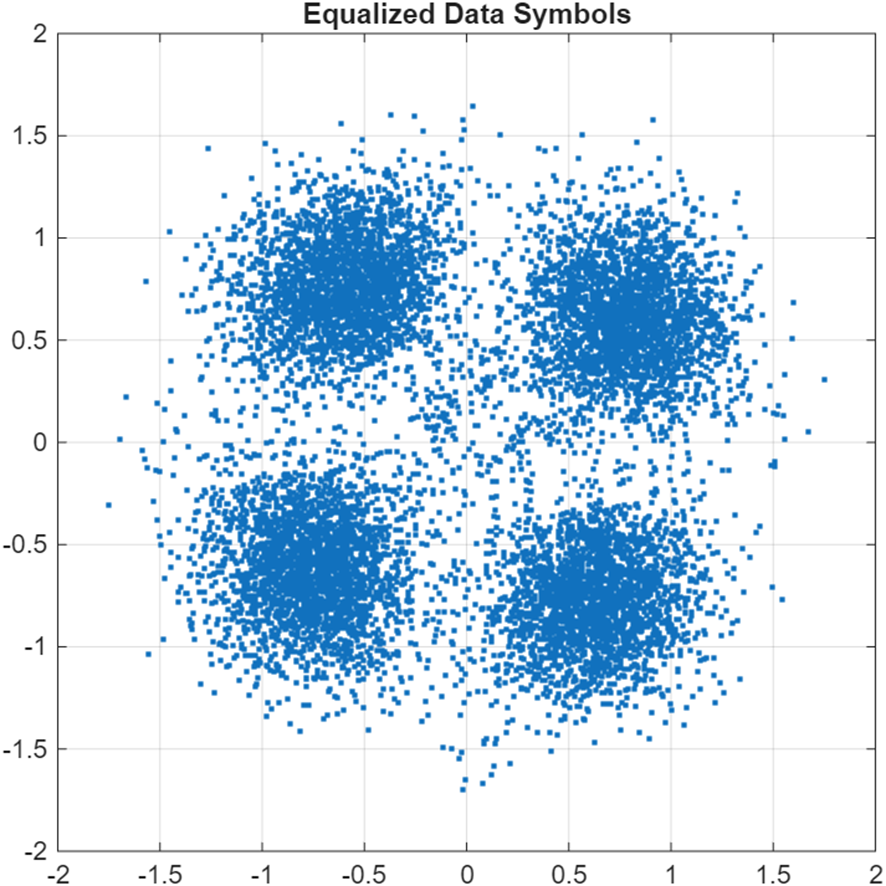
\includegraphics[width=0.45\textwidth]{figures/chap3_channel/c4_3.png} \\
        \small (a) Initial Equalized Symbols & \small (b) Improved Sideband Reception
    \end{tabular}
    \caption[Channel 4: Band-Rejection Equalization Comparison]{%
        Comparison of received 4-QAM constellations for Channel 4: (a) High BER reception due to band-rejection characteristics; 
        (b) Improved constellation achieved by activating sideband subcarriers, leading to lower bit error rates.
    }%
    \label{fig:ch4_constellations}%
\end{figure}

Additionally, \Cref{fig:ch4_correlation} illustrates the signal magnitude and the normalized correlation metric used for frame detection in this band-limited scenario.

\section{Channel 5: Multipath Fading} \label{sec:Channel5}

Channel 5 exhibits the characteristics of a typical multipath environment.
The time-domain view shows a sequence of taps with exponentially decaying amplitudes, representing discrete signal paths with varying delays and attenuations.
The PDP and frequency response are detailed in \Cref{fig:ch5_pdp_analysis} and \Cref{fig:ch5_numerical_summary}.

Consistent with our methodology, the raw LS estimate is noisy.
By applying a window to the impulse response, we obtain a smoothed frequency response that mitigates noise enhancement.
\Cref{fig:ch5_ber_performance} compares the BER performance across different strategies:
\begin{itemize}
    \item \textbf{No Equalization}: Results in a BER of 0.5 (failure).
    \item \textbf{LS Equalization}: Provides functional performance but remains suboptimal due to noise.
    \item \textbf{MMSE (Window $L=15$)}: Yields the best performance, as the window length matches the significant channel taps.
    \item \textbf{MMSE (Window $L=150$)}: Performance degrades and approaches the LS curve, as the wide window admits excessive noise.
\end{itemize}

\begin{figure}[!ht]
    \centering
    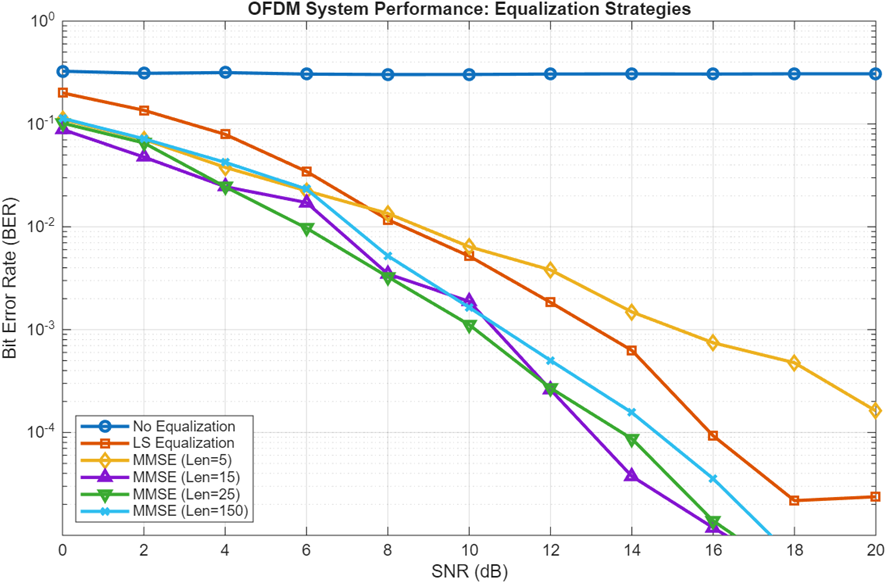
\includegraphics[width=0.85\textwidth]{figures/chap3_channel/c5_2.png}
    \caption[Channel 5: BER Performance Comparison]{%
        Bit Error Rate (BER) performance curves for Channel 5. The plot compares the performance of an unequalized system, LS equalization, and MMSE equalization with varying filter lengths ($L=5, 15, 25, 150$).
    }%
    \label{fig:ch5_ber_performance}%
\end{figure}

For a visual confirmation of the equalization success, the recovered 4-QAM constellation is provided in \Cref{fig:ch5_constellation} in the appendix.


\begin{idea}[Optimization Proposal: Adaptive Cyclic Prefix]
    The Cyclic Prefix (CP) is a critical mechanism to mitigate Inter-Symbol Interference (ISI), yet its standard configuration often incurs unnecessary overhead.
    Per the project specifications, a fixed CP length of $N_{\text{CP}} = 256$ samples is mandated for an OFDM symbol size of $N = 512$ subcarriers. While robust, this results in a significant efficiency loss of approximately $1/3$ of the transmission time.
    
    To address this, we propose an adaptive CP strategy based on the effective Channel Impulse Response (CIR) length.
    Our experimental results confirm that efficiency can be maximized without compromising signal integrity by tailoring the CP to each specific channel:
    \begin{itemize}
        \item \textbf{Channels 1 \& 2 (Flat Fading):} As these channels exhibit negligible delay spread, the CP can be drastically reduced to a single sample (or removed entirely), maximizing data throughput.
        \item \textbf{Channel 5 (Multipath):} A reduced CP of approximately 15 samples suffices to cover the delay spread, significantly lower than the default 256.
        \item \textbf{Channel 3 (High Dispersion):} Due to the severe delay spread, retaining the full CP length is necessary to prevent ISI.
    \end{itemize}
    This tailored approach ensures that the system operates at maximum efficiency for the given physical channel conditions.
\end{idea}
\setcounter{chapter}{3}
\chapter{System Performance} \label{ch:performance}

Spectral efficiency is a key performance metric for multicarrier systems such as OFDM, as it quantifies how efficiently the available bandwidth is used to transmit useful information. It is formally defined as the number of successfully transmitted information bits per second per Hertz (bit/s/Hz). In this project, this metric serves to evaluate the trade-offs introduced by modulation order, coding rates, frame structure, and the various overheads inherent to the OFDM physical layer.

\section{Analytical Framework}

For the implemented OFDM system, the spectral efficiency $\eta$ is derived by accounting for the modulation order, coding gains, and structural overheads. The analytical expression is formulated as follows:

\begin{equation} \label{eq:spectral_efficiency_full}
    \eta = \mathrm{BPS} \cdot R_{\mathrm{FEC}} \cdot \underbrace{\frac{N_{\mathrm{data}}}{N_{\mathrm{carr}}}}_{\text{Subcarrier use}} \cdot \underbrace{\frac{N_{\mathrm{carr}}}{N_{\mathrm{carr}} + N_{\mathrm{cp}}}}_{\text{Guard interval}} \cdot \underbrace{\frac{N_{\mathrm{data\_sym}}}{N_{\mathrm{data\_sym}} + N_{\mathrm{training\_sym}}}}_{\text{Protocol overhead}} \eqend
\end{equation}

In this expression, $\mathrm{BPS}$ denotes the bits per symbol, $R_{\mathrm{FEC}}$ is the forward error correction rate, and the subsequent ratios represent the losses due to unused edge subcarriers, the cyclic prefix (CP), and the training symbols required for synchronization and channel estimation.

\section{Spectral Efficiency Trends and Trade-offs}

The efficiency of the system is sensitive to several design parameters, each presenting a fundamental compromise between throughput and link robustness.

\begin{remark}[Modulation and Bandwidth]
    Increasing the modulation order grows spectral efficiency logarithmically; however, higher-order constellations require significantly higher SNR to maintain acceptable bit error rates in noisy acoustic channels. Conversely, while increasing the occupied bandwidth scales the achievable data rate, the spectral efficiency remains unchanged, as the number of transmitted bits per Hertz is a property of the multicarrier structure itself.
\end{remark}

\begin{figure}[!ht]
    \ffigbox[\FBwidth]{%
        \begin{tabular}{cc}
            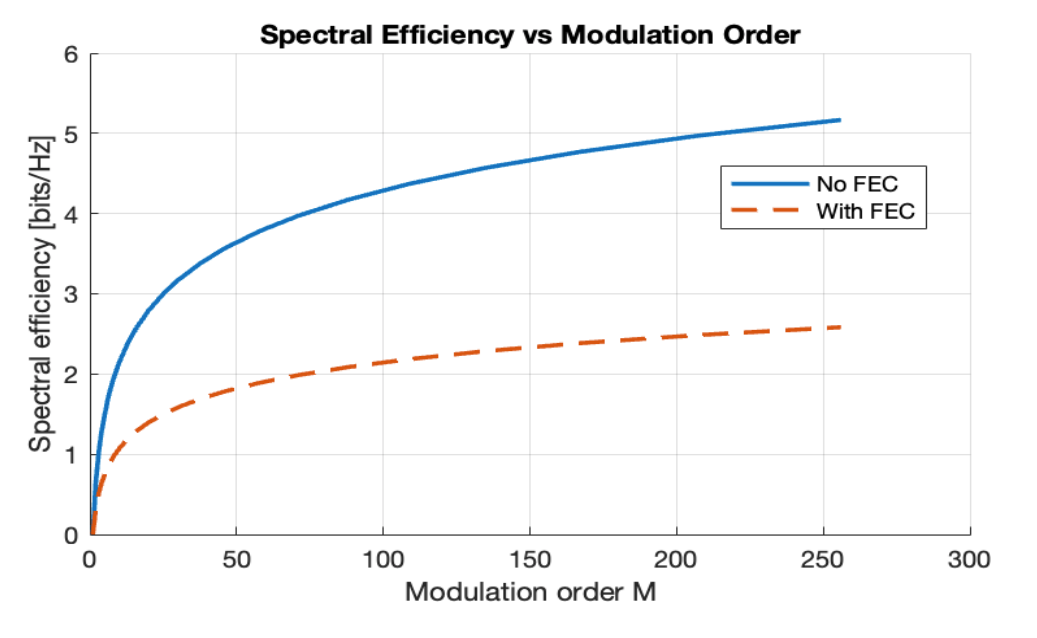
\includegraphics[width=0.45\textwidth]{figures/chap4_performance/Spectral_Efficiency_vs_Modulation_Order.png} & 
            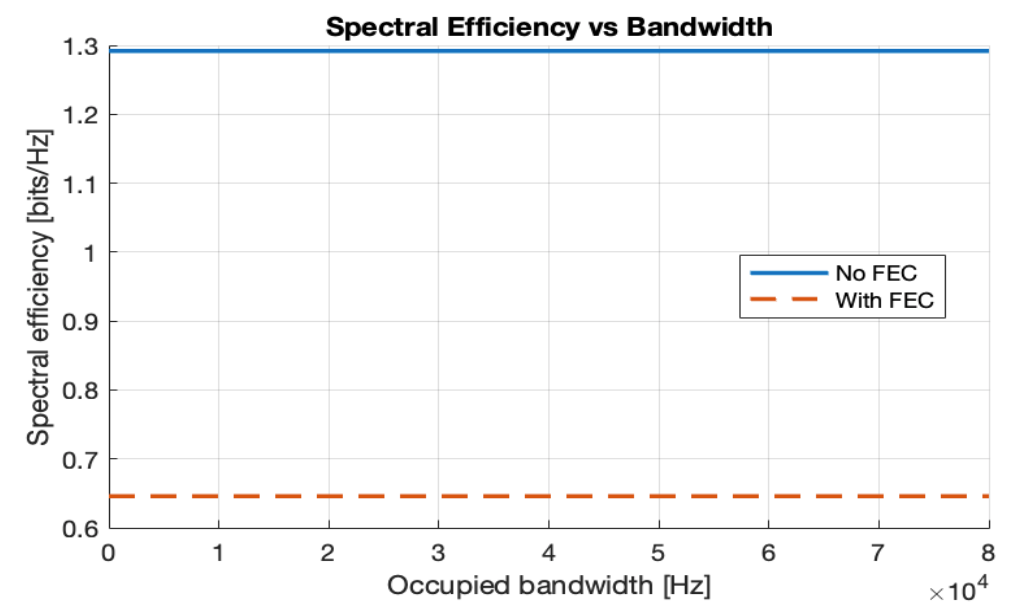
\includegraphics[width=0.45\textwidth]{figures/chap4_performance/Spectral_Efficiency_vs_Bandwidth.png} \\
        \end{tabular}
    }{%
        \caption[Modulation and Bandwidth Trends]{%
            (Left) Logarithmic growth of $\eta$ with modulation order. (Right) Constant spectral efficiency across varying bandwidths, illustrating the inherent behavior of multicarrier systems.
        }%
        \label{fig:eta_trends_basic}%
    }
\end{figure}

The temporal and frequency overheads also dictate the system's performance limits. Increasing the number of subcarriers $N_{\mathrm{carr}}$ improves efficiency by amortizing fixed overheads, though this gain saturates as the relative impact of unused carriers becomes negligible. In the time domain, the cyclic prefix is essential to preserve orthogonality in multipath environments, but it introduces a linear reduction in $\eta$ as its length $N_{\mathrm{cp}}$ increases.



\begin{figure}[!ht]
    \ffigbox[\FBwidth]{%
        \begin{tabular}{cc}
            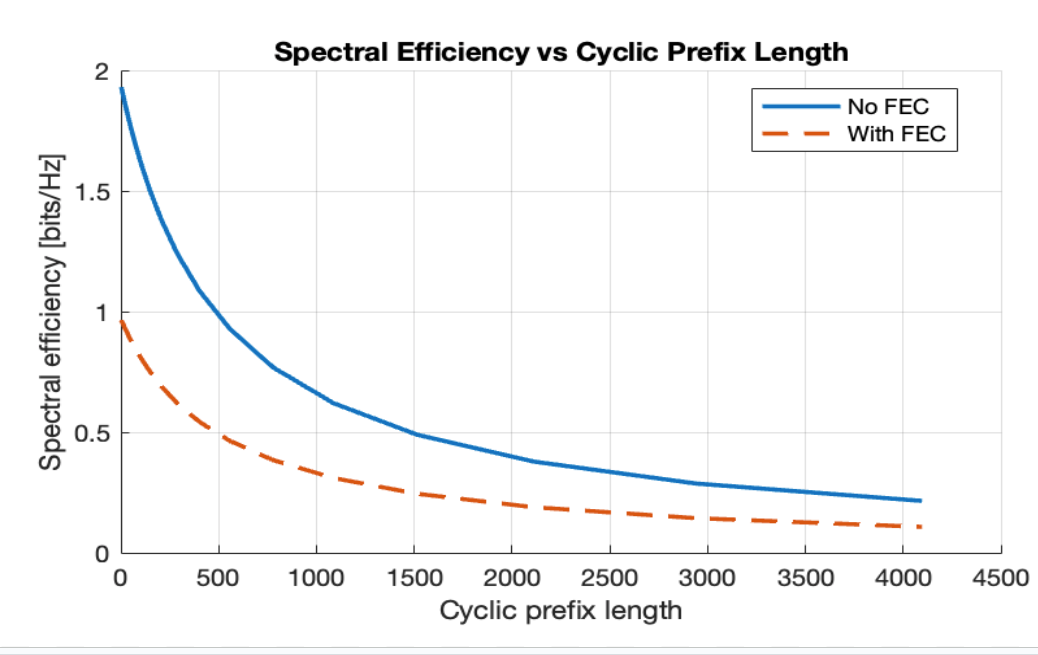
\includegraphics[width=0.45\textwidth]{figures/chap4_performance/Spectral_Efficiency_vs_Cyclic_Prefix_Length.png} & 
            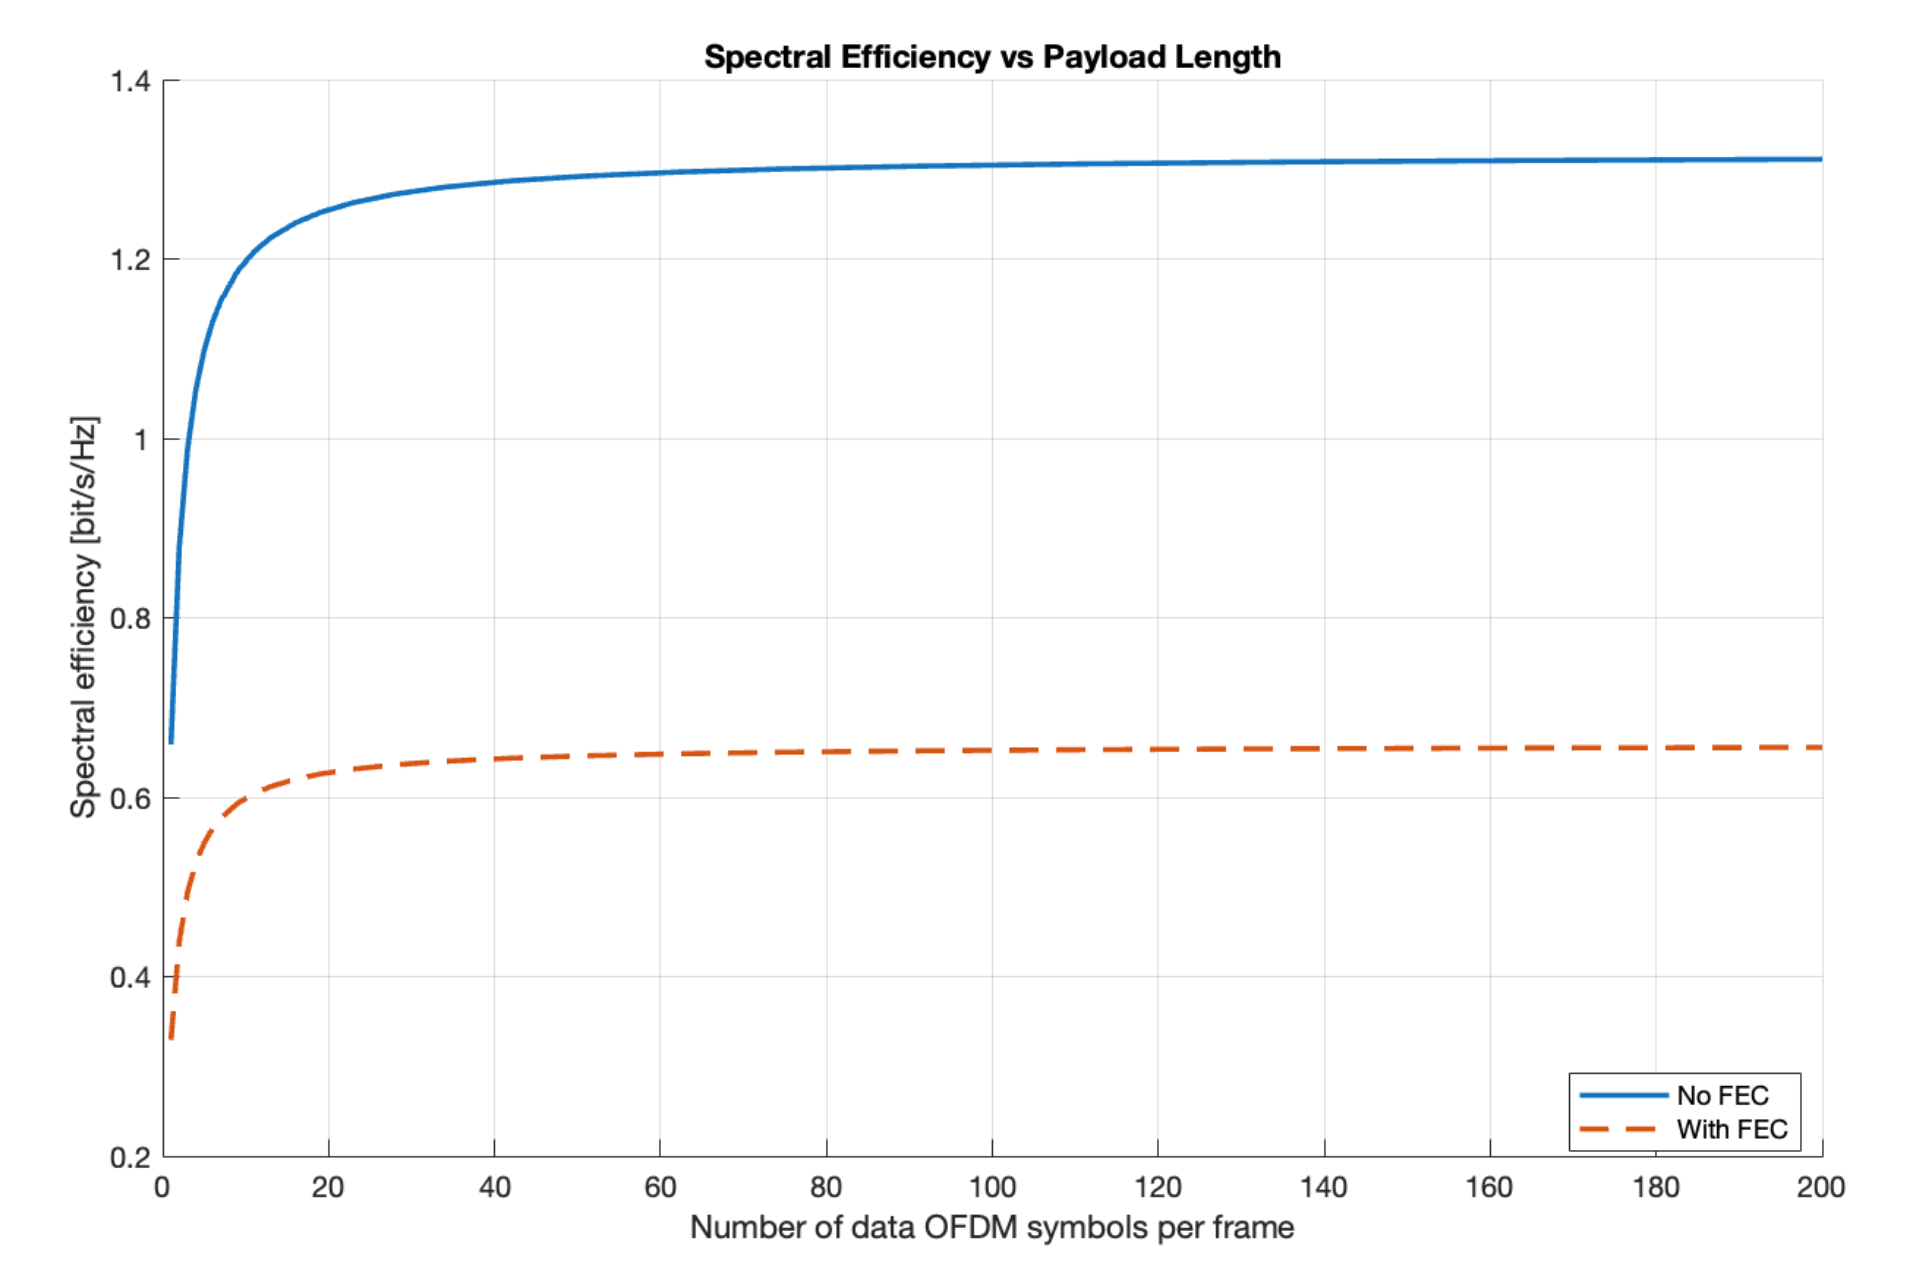
\includegraphics[width=0.45\textwidth]{figures/chap4_performance/Spectral_Efficiency_vs_Payload_Length.png} \\
        \end{tabular}
    }{%
        \caption[Temporal Overhead Impact]{%
            Effect of the cyclic prefix length and payload duration on efficiency. Longer payloads amortize the training symbol overhead, allowing $\eta$ to converge toward its theoretical upper bound.
        }%
        \label{fig:eta_overhead_trends}%
    }
\end{figure}

\begin{Note}[Amortization of Training Symbols]
    Training symbols are indispensable for synchronization, yet they reduce the fraction of useful data. As payload length increases, this overhead is amortized, motivating the use of long frames whenever the acoustic channel remains stationary.
\end{Note}

\section{Summary}

The spectral efficiency analysis highlights the fundamental design choices of the project. While higher modulation orders and larger payloads improve the bit/s/Hz ratio, the environmental constraints of the Rolex Learning Center—specifically multipath dispersion and noise—necessitate the use of cyclic prefixes and FEC. The final system parameters represent a calculated balance, ensuring reliable transmission at a sustainable information density.
%\setcounter{chapter}{13} % "N" (14th letter, but latex first increments -> 14-1=13)
\chapter{Real Acoustic Transmission} \label{ch:transmission}

The communication system was validated through a practical experiment involving the transmission of a color image within the Rolex Learning Center.
This environment presents a realistic acoustic scenario characterized by a large open space, carpeted flooring, and glass walls, introducing specific propagation challenges.

\section{Experimental Setup and Channel Analysis}

The physical configuration consisted of a transmitter (loudspeakers) and a receiver (laptop microphone) separated by a considerable distance.
As illustrated in \Cref{fig:trans_setup} (see \Cref{ch:appendix_visual}), the geometry of the setup allows us to visually identify potential signal paths: the direct line-of-sight, a reflection off the laptop chassis, and a longer reflection from the adjacent glass wall.

\begin{figure}[!ht]
    \fcapside[\FBwidth]{%
        \captionsetup{parskip = .5\baselineskip plus 1pt}%
        \caption[]{%
             Physical experimental setup showing the acoustic transmission environment.
        }%
        \label{fig:ch5_physical}%
    }{%
        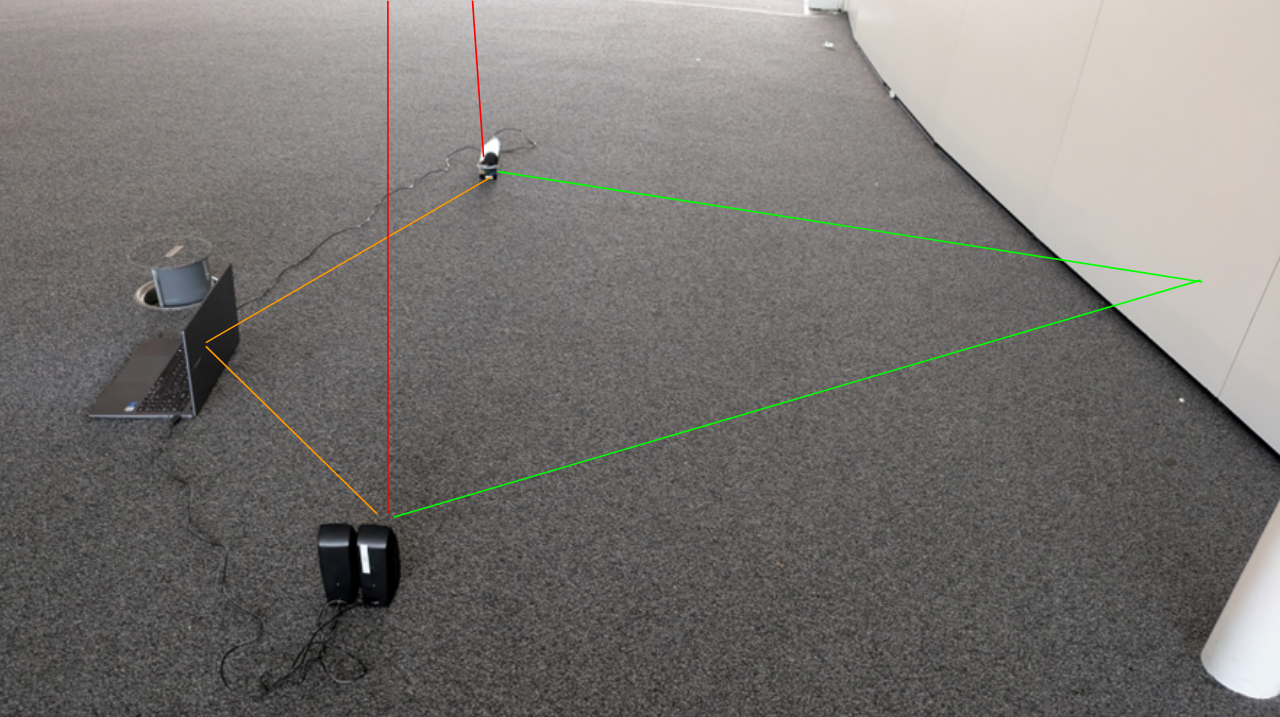
\includegraphics[width=0.70\textwidth]{figures/chap5_transmission/imag1.png}
    }
\end{figure}

The increased distance between the transmitter and receiver results in significant signal attenuation due to the exponential decay of acoustic energy, thereby reducing the Signal-to-Noise Ratio (SNR) and potentially increasing the Bit Error Rate (BER).
Despite these adverse conditions, the channel estimation performed using the methodology described in \Cref{ch:channel} successfully captured the multipath profile.

Analysis of the Impulse Response, detailed in \Cref{fig:trans_cir_pdp} in the appendix, reveals a sparse channel structure dominated by three primary components:
\begin{itemize}
    \item \textbf{Tap 1:} The direct path, carrying the highest energy.
    \item \textbf{Tap 2:} A short-delay reflection, likely attributable to the laptop screen or keyboard.
    \item \textbf{Tap 4:} A delayed component, corresponding to the reflection from the distant glass wall.
\end{itemize}

Following the strategy defined in the previous chapter, we applied a practical MMSE windowing technique to truncate the impulse response, retaining only these significant taps to minimize noise injection during equalization. The corresponding LMMSE report is available in \Cref{fig:trans_lmmse_report}.

\section{Image Transmission Challenges}

Transmitting image data introduces specific challenges compared to continuous data streams, primarily regarding temporal stability and data integrity.

\subsection{Signal Fragmentation}
The transmission of a high-resolution image requires a signal duration of several seconds.
In a real acoustic environment, the channel is potentially time-varying (e.g., due to movement or temperature fluctuations).
If the entire image were transmitted as a single block, the channel estimate obtained at the preamble could become stale by the end of the packet, leading to equalization errors.

To mitigate this, the image was fragmented into 10 independent frames.
Each frame carries its own preamble and training symbol, forcing a re-estimation of the channel for every segment.
This ensures that the equalization coefficients remain valid for the duration of the frame, adapting to any slow variations in the environment.

\subsection{Data Sensitivity and Formats}
We utilized the Bitmap (BMP) format for transmission.
Unlike compressed formats (e.g., JPEG), where a single bit error can destroy the entropy coding and render the image unreadable, Bitmaps are more resilient to payload errors.
However, they still rely on a critical \textbf{file header} to define dimensions and color depth.

\begin{remark}[The Header Problem]
    If the file header is corrupted by noise or deep fading, the receiver cannot reconstruct the pixel grid, resulting in a total failure to display the image.
    While our current implementation successfully retrieved the image (as shown in \Cref{fig:result_image}), the risk of header corruption suggests the need for robust protection.
\end{remark}

\begin{figure}[!ht]
    \centering
    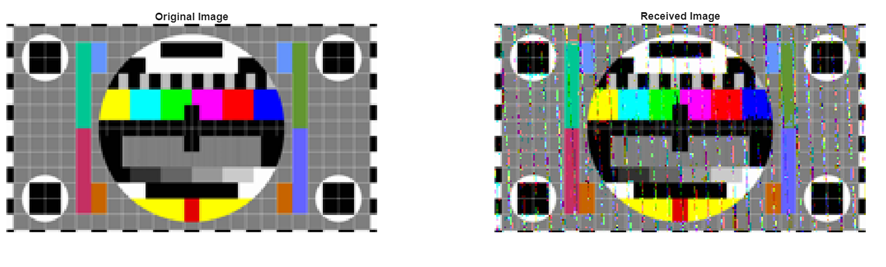
\includegraphics[width=0.85\textwidth]{figures/chap5_transmission/imag5.png}
    \caption[Transmission Results]{Comparison between the original transmitted test pattern and the received image. The system successfully recovered the color information despite the multipath environment, with a measured BER of \num{0.094}.}
    \label{fig:result_image}
\end{figure}

The visual result confirms the viability of the equalization scheme.
However, to ensure reliability in cases where the BER spikes, it is necessary to implement Forward Error Correction (FEC), particularly to protect critical metadata such as image headers.
This optimization is the subject of the following chapter.

\subsection{Peak-to-Average Power Ratio (PAPR) and Nonlinearities}
\label{sub:PAPR}

A significant drawback of the OFDM modulation used in this acoustic transmission is the high Peak-to-Average Power Ratio (PAPR), a characteristic that becomes particularly problematic when transmitting structured data like images. In our experiment, if the image data contains repetitive patterns—such as large areas of a single color in a BMP file—the transmitted symbols $A[k]$ become highly correlated. When these symbols are processed by the Inverse Fast Fourier Transform (IFFT), they may align in phase, resulting in constructive interference that produces large instantaneous power peaks.

The continuous-time baseband OFDM signal can be expressed mathematically as the sum of $N$ orthogonal subcarriers:
\begin{equation} \label{eq:ofdm_signal_papr}
    s(t) = \frac{1}{\sqrt{N}} \sum_{k=0}^{N-1} A[k] \E^{\I 2\pi k \Delta f t} \eqcomma \quad 0 \le t \le T \eqend
\end{equation}
The PAPR is defined as the ratio between the maximum instantaneous power and the average power of the signal:
\begin{equation} \label{eq:papr_formula}
    \text{PAPR}\{s(t)\} \doteq \frac{\max_{0 \le t \le T} |s(t)|^{2}}{\mathbb{E}\left[|s(t)|^{2}\right]} \eqend
\end{equation}

In a typical acoustic scenario, these power spikes are detrimental for several reasons. First, if the peaks exceed the linear dynamic range of the loudspeaker's power amplifier or the digital-to-analog converter (DAC), the signal is clipped, leading to severe nonlinear distortion. This clipping introduces "spectral regrowth," which generates out-of-band interference, but more critically, it creates in-band distortion. This effect manifests as an additional noise floor that degrades the constellation points, as seen in the spread of symbols in \Cref{fig:ch5_ber_performance} (a), and unlike Gaussian noise, it cannot be fully mitigated by the LMMSE equalizer alone.



To mitigate this effect during the Rolex Learning Center trials, the digital gain was backed off (Input Back-Off) to ensure the peaks remained within the linear region of the hardware. While this prevents nonlinear distortion, it simultaneously reduces the average signal power, leading to a lower Signal-to-Noise Ratio (SNR) at the receiver. This trade-off explains why certain frames exhibited higher BER despite successful channel estimation, as the system operated with reduced power margins to accommodate these PAPR spikes.
\chapter{Channel Coding \& System Performance} \label{ch:coding}

To enhance system robustness against the adverse conditions of the acoustic channel, we implement a Forward Error Correction (FEC) strategy. While this introduces a trade-off in terms of reduced throughput and increased computational complexity, it is essential for maintaining a reliable link in low SNR regimes.

\section{Concatenated FEC Architecture} \label{sec:FEC_Architecture}

The architecture follows a classical hierarchical structure, employing an outer block code and an inner convolutional code. See \textcite{LinCostello2004}. This configuration is synergistic: the inner decoder suppresses the noise floor, while the outer decoder cleans up the residual error bursts that often escape the inner stage.

\begin{definition}[Concatenated Code Specification]
    The implemented scheme consists of two layers:
    \begin{itemize}
        \item \textbf{Outer Code:} A Reed-Solomon (RS) block code with parameters $(n,k) = (255, 239)$ operating on $m=8$-bit symbols. This code can correct up to $t=8$ symbol errors per block.
        \item \textbf{Inner Code:} A convolutional code with rate $R=1/2$ and constraint length $K=7$. It utilizes the standard generator polynomials $G_1 = 171_8$ and $G_2 = 133_8$.
    \end{itemize}
    This results in a net coding rate of approximately $R_{net} \approx 0.47$, prioritizing reliability over spectral efficiency.
\end{definition}

\begin{figure}[!ht]
    \fcapside[\FBwidth]{%
        \captionsetup{parskip = .5\baselineskip plus 1pt}%
        \caption[BER Performance Comparison]{%
            Bit Error Rate (BER) versus SNR.
            The plot illustrates the \enquote{coding gain} achieved by the concatenated scheme. The waterfall region typically begins around 10 dB, where the Viterbi decoder becomes effective against random noise.
        }%
        \label{fig:ber_fec}%
    }{%
        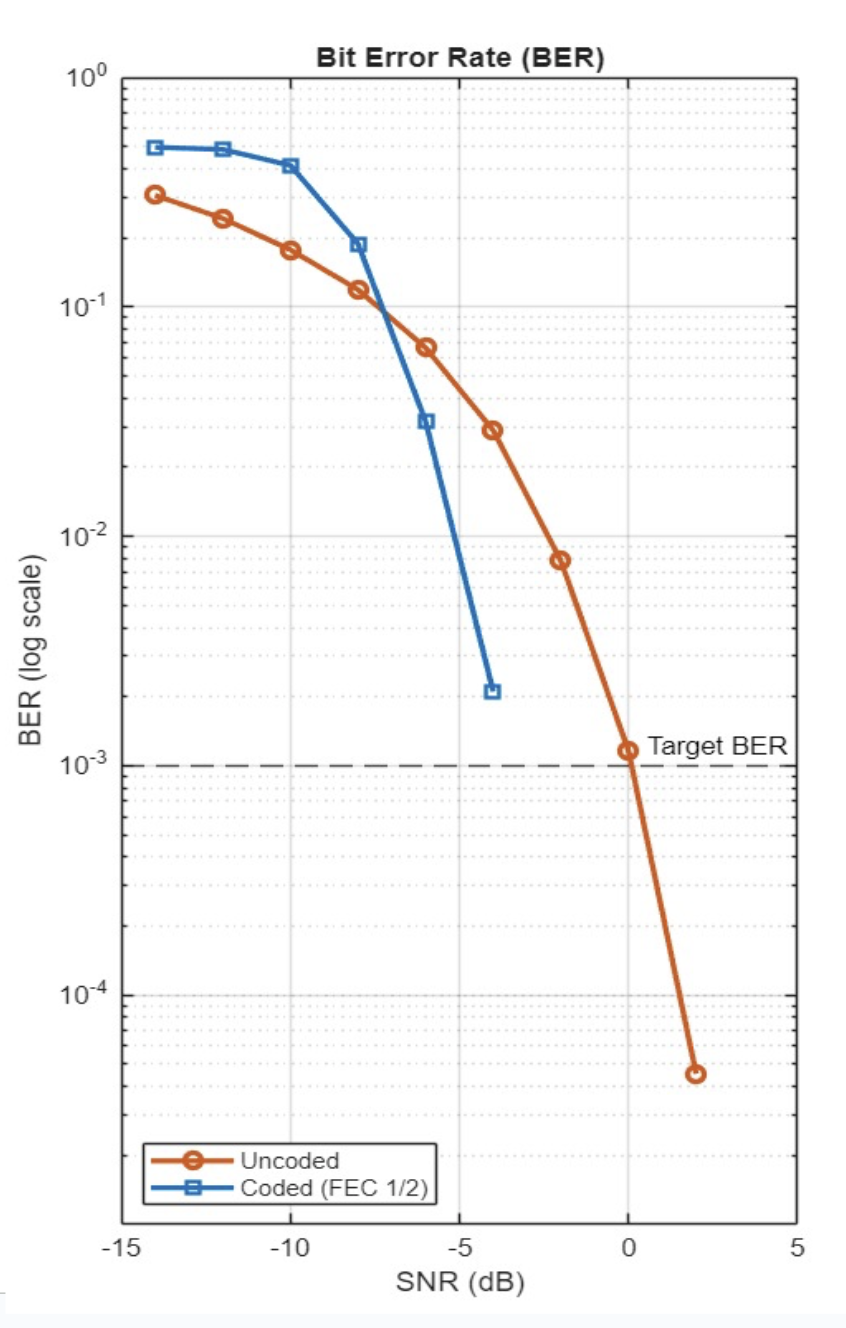
\includegraphics[width=0.45\textwidth]{figures/chap4_performance/Spectral_Efficiency_BER.png}
    }
\end{figure}

\section{Implementation Logic} \label{sec:Coding_Implementation}

The data processing flow is orchestrated by the \path{custom_function/transmit/channel_encoder.m} and \path{custom_function/receive/channel_decoder.m} scripts. These functions manage the alignment between the bit-level operations of the convolutional code and the symbol-level operations of the RS code.

\subsection{Encoding Process}

At the transmitter, the payload bits undergo a strict formatting sequence:
\begin{enumerate}
    \item \textsf{Symbol Alignment:} Input bits are padded to ensure the total length is a multiple of $m=8$, then converted into integer symbols.
    \item \textsf{Outer Encoding:} The \path{rsenc} function processes blocks of $k=239$ symbols, appending parity data to form $(n,k)$ codewords.
    \item \textsf{Inner Encoding:} The symbol stream is serialized back into bits and passed through the \path{convenc} function, generating the final redundant bitstream for modulation.
\end{enumerate}

\subsection{Decoding and Recovery}

The receiver performs the inverse operations with specific safeguards to maximize data integrity. The inner decoding uses the Viterbi algorithm (\path{vitdec}) in \emph{hard-decision} mode, with a traceback depth defined by \path{conf.coding.traceBackDepth} (typically $5K$ to $7K$).

\begin{remark}[Fallback Mechanism]
    A critical feature of our \path{channel_decoder.m} is the robustness against decoding failures.
    If the Reed-Solomon decoder detects more errors than its correction capability $t$, it typically fails.
    In our implementation, we catch this failure and extract the \emph{systematic part} of the block (the raw data symbols) instead of discarding the frame entirely. This allows upper layers to potentially recover partial information.
\end{remark}

\section{Performance Analysis} \label{sec:Performance_Analysis}

The impact of the FEC chain is quantified in \Cref{fig:ber_fec}. The transition from uncoded to coded transmission yields a significant coding gain.
In the acoustic channel, where multipath fading creates severe spectral nulls, the uncoded BER curve often flattens (error floor). The concatenated code effectively lowers this floor.

\begin{Note}[Hard vs. Soft Decision]
    The current implementation utilizes \emph{hard-decision} Viterbi decoding.
    Transitioning to \emph{soft-decision} decoding—passing confidence levels from the demodulator to the decoder—would theoretically yield an additional gain of 2 dB to 3 dB, though at the cost of increased memory usage and complexity.
\end{Note}

\Cref{tab:coding_summary} summarizes the trade-offs observed during system characterization.

\begin{table}[!ht]
    \centering
    \small
    \begin{tblr}{
        colspec = {X[l,m] X[c,m] X[c,m]},
        hlines, vlines,
        row{1} = {bg=gray!15, font=\sffamily\bfseries}
    }
        Metric & Uncoded System & Coded System \\
        Primary Error Type & Random Bit Flips & Residual Symbol Bursts \\
        Spectral Efficiency & High ($1.0 \times$ rate) & Low ($\approx 0.47 \times$ rate) \\
        Throughput @ High SNR & Max & Reduced \\
        Throughput @ Low SNR & Near Zero (Packet Loss) & Maintained \\
        Decoder Complexity & Negligible & High (Viterbi + RS) \\
    \end{tblr}
    \caption[Coding Trade-offs]{Comparison of link characteristics with and without the Concatenated FEC scheme.}
    \label{tab:coding_summary}
\end{table}
%\chapter{Code Organisation} \label{ch:code}

\begin{figure}[!ht]
    \fcapside[\FBwidth]{%
        \captionsetup{parskip = .5\baselineskip plus 1pt}%
        \caption[Project File Structure and Usage]{%
            \textbf{Structure and Usage Guide.}
            
            The project code is organized into a root directory containing the execution scripts and configuration, with modular functions separated by purpose.
            
            \textbf{Execution Flow:} The main entry point is \path{main.m}, which runs the complete image transmission experiment. It loads the image from \path{img/}, encodes it, transmits it (via audio or emulator), and reconstructs the received result. For performance analysis, \path{main_channelPlot.m} generates BER curves vs SNR, while \path{main_equalizationComp.m} compares different equalizer settings.
            
            \textbf{Configuration:} All system parameters are centralized in \path{configurations.m}. This includes the OFDM setup (512 subcarriers, CP length), signal parameters ($f_s=48$kHz), and channel model selection. Modify this file to change the experiment conditions.
            
            \textbf{Core Modules:} The \path{custom_function/} directory houses the user-implemented logic. It is split into \path{transmit/} (encoder, frame builder) and \path{receive/} (synchronization, channel estimation, decoding). Helper scripts like \path{preamble_generate.m} reside in the root of this folder. The \path{provided_function/} directory contains the pre-compiled channel emulator and standard filters provided for the course.
        }%
        \label{fig:project-structure}%
    }{%
        \begin{tikzpicture}[dirtree]
            \node[directory] {OFDM Project/}
            child { node {configurations.m}}
            child { node {main.m}}
            child { node {main\_channelPlot.m}}
            child { node {main\_equalizationComp.m}}
            child { node[directory] {custom\_function/}
                child { node {preamble\_generate.m}}
                child { node {tfplotReImPhase.m}}
                child { node[directory] {receive/}
                    child { node {receiver.m}}
                    child { node {estimateTauAndCFO.m}}
                    child { node {ChannelMetrics.m}}
                    child { node {channel\_estLS.m}}
                    child { node {channel\_decoder.m}}
                    child { node {correctOFDMSymbolRotation.m}}
                    child { node {ofdm\_rx\_frame.m}}
                }
                child [missing] {} child [missing] {} child [missing] {} child [missing] {} child [missing] {} child [missing] {} child [missing] {} 
                child { node[directory] {transmit/}
                    child { node {transmitter.m}}
                    child { node {ofdm\_tx\_frame\_with\_pilots.m}}
                    child { node {channel\_encoder.m}}
                }
            }
            child [missing] {} child [missing] {} child [missing] {} child [missing] {} child [missing] {} child [missing] {} child [missing] {} child [missing] {} child [missing] {} child [missing] {} child [missing] {} child [missing] {}
            child [missing] {} child [missing] {}
            child { node[directory] {img/}
                child { node {test-image.bmp}}
                child { node {received\_image.bmp}}
            }
            child [missing] {}
            child { node[directory] {provided\_function/}
                child { node {channel\_emulator.p}}
                child { node {ofdmlowpass.m}}
                child { node {rrc.m}}
                child { node {ofdm\_rx\_resampling.m}}
                child { node {ofdm\_tx\_resampling.m}}
            }
            ;
        \end{tikzpicture}%
    }
\end{figure}







%\chapter{TEST} \label{ch:test}

Ready to test some things?
%\chapter{ISI}

\section{Mathematical Derivation of ISI Quantification}

Starting from the discrete equivalent channel model with cursor $p[d]$, we derive the error bound step-by-step:

\begin{align}
    q[n]        &= \sum_{k} p[k] A[n-k] + z[n] \\
    q[n]        &= p[d] A[n-d] + \sum_{k \neq d} p[k] A[n-k] + z[n] \\
    \left| \frac{q[n]}{p[d]} - A[n-d] \right| &= \left| \sum_{k \neq d} \frac{p[k]}{p[d]} A[n-k] + \frac{z[n]}{p[d]} \right| \\
    \left| \frac{q[n]}{p[d]} - A[n-d] \right| &\le |A|_{\text{max}} \underbrace{\sum_{k \neq d} \frac{|p[k]|}{|p[d]|}}_{D_{\text{peak}}} + \frac{|z[n]|}{|p[d]|} \\
    \left|\frac{q[n]}{p[d]} - A[n-d] \right| &\le \gamma_{\text{ISI}} \left( \frac{d_{\text{min}}}{2} \right) + \frac{|z[n]|}{|p[d]|}
\end{align}


\begin{align}
\gamma_{\text{ISI}} &\doteq D_{\text{peak}} / \eta\\
D_{\text{peak}} &\doteq \sum_{k \neq d} \frac{|p[k]|}{|p[d]|} \\
\eta &\doteq \frac{d_{\text{min}}/2}{|A|_{\text{max}}}
\end{align}

\newpage
\begin{align}
    q[n] &= \sum_{k} p[k] A[n-k] + z[n] && \text{\small (Discrete Model)} \nonumber \\
    &= p[d] A[n-d] + \sum_{k \neq d} p[k] A[n-k] + z[n] && \text{\small (Cursor Decomposition)} \nonumber \\[1em]
    \frac{q[n]}{p[d]} &= A[n-d] + \sum_{k \neq d} \frac{p[k]}{p[d]} A[n-k] + \frac{z[n]}{p[d]} && \text{\small (Normalization)} \nonumber \\[1em]
    \left| \frac{q[n]}{p[d]} - A[n-d] \right| &= \left| \sum_{k \neq d} \frac{p[k]}{p[d]} A[n-k] + \frac{z[n]}{p[d]} \right| && \text{\small (Error Definition)} \nonumber \\
    &\le \sum_{k \neq d} \left| \frac{p[k]}{p[d]} \right| |A[n-k]| + \left| \frac{z[n]}{p[d]} \right| && \text{\small (Triangle Inequality)} \nonumber \\[1em]
    &\le |A|_{\text{max}} \underbrace{\sum_{k \neq d} \frac{|p[k]|}{|p[d]|}}_{D_{\text{peak}}} + \frac{|z[n]|}{|p[d]|} && \text{\small (Worst Case Distortion)} \nonumber \\[1em]
    &\le |A|_{\text{max}} \left( \gamma_{\text{ISI}} \frac{d_{\text{min}}/2}{|A|_{\text{max}}} \right) + \frac{|z[n]|}{|p[d]|} && \text{\small (Substituting } D_{\text{peak}} = \gamma_{\text{ISI}}\eta \text{)} \nonumber \\[1em]
    \therefore \quad \left| \frac{q[n]}{p[d]} - A[n-d] \right| &\le \gamma_{\text{ISI}} \left( \frac{d_{\text{min}}}{2} \right) + \frac{|z[n]|}{|p[d]|} && \text{\small (Final Bound)}
\end{align}
%\include{chapters/Usage}
%\include{chapters/Features}
%\include{chapters/Tips}

\backmatter
%\include{chapters/Summary}

\appendix
%\include{chapters/Appendix}
\chapter{Appendix of Images} \label{ch:appendix_visual}


\begin{figure}[!ht]
    \fcapside[\FBwidth]{%
        \captionsetup{parskip = .5\baselineskip plus 1pt}%
        \caption[]{%
             Power Delay Profile (PDP) utilized for discrete channel modeling.
        }%
        \label{fig:ch2_pdp}%
    }{%
        
\includegraphics[width=0.40\textwidth]{figures/chap3_channel/1.png}
    }
\end{figure}

\section{Channel 1}

\begin{figure}[!ht]
    \centering
    \captionsetup{parskip = .5\baselineskip plus 1pt}
    \begin{tabular}{ccc}
        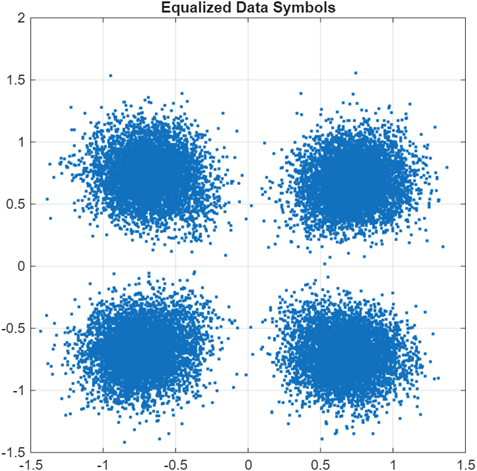
\includegraphics[width=0.3\textwidth]{figures/chap3_channel/c1_3.png} &
        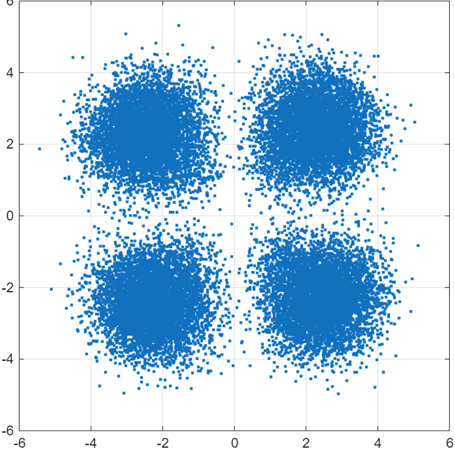
\includegraphics[width=0.3\textwidth]{figures/chap3_channel/c1_4.png} &
        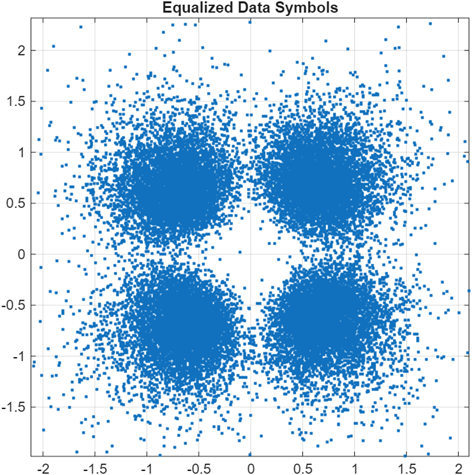
\includegraphics[width=0.3\textwidth]{figures/chap3_channel/c1_2.png} \\
        \small (a) MMSE Equalization & \small (b) LS Equalization & \small (c) No Equalization
    \end{tabular}
    \caption[Channel 1: Comparison of Equalization Techniques]{%
        Constellation comparison for Channel 1: (a) MMSE equalization provides optimal clustering; 
        (b) LS equalization shows higher noise sensitivity; 
        (c) Unequalized signal exhibiting an open eye pattern due to low ISI levels.
    }%
    \label{fig:ch1_constellation_comparison}%
\end{figure}


\begin{figure}[!ht]
    \ffigbox[\FBwidth]{%
        \begin{tabular}{cc}
            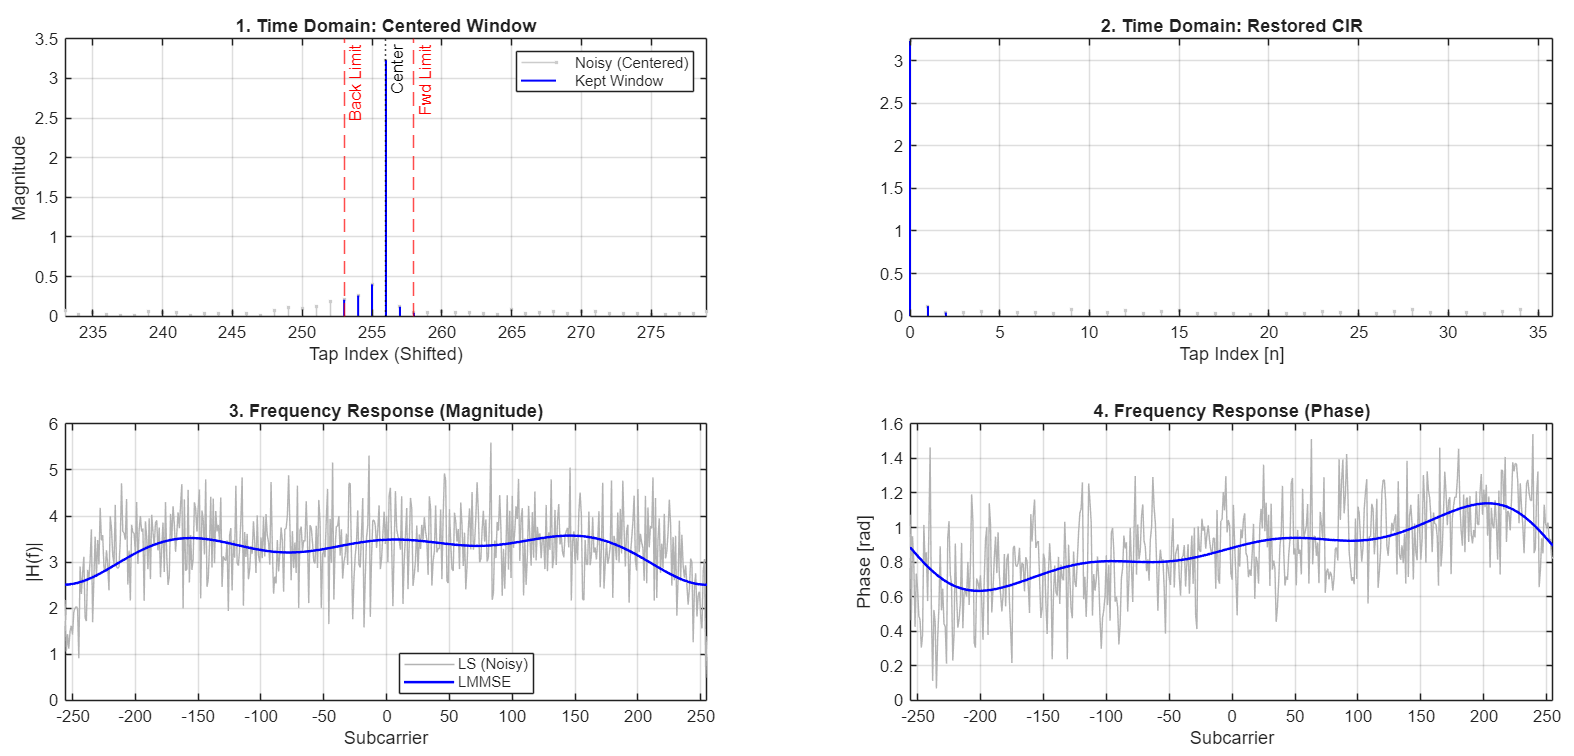
\includegraphics[width=0.67\textwidth]{figures/chap3_channel/c1_1.png} & 
            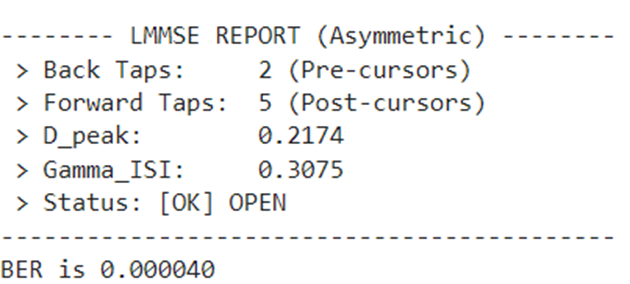
\includegraphics[width=0.27\textwidth]{figures/chap3_channel/c1_5.png} \\
        \end{tabular}
    }{%
        \caption[Channel 1: Estimation and ISI Report]{%
            (Left) Time domain CIR windowing and Frequency Response analysis for Channel 1. 
            (Right) LMMSE numerical report with $\gamma_{\text{ISI}} = 0.3075$, confirming an open eye status ([OK] OPEN).
        }%
        \label{fig:ch1_channel_estimation_summary}%
    }
\end{figure}

\newpage
\section{Channel 2}

\begin{figure}[!ht]
    \centering
    \captionsetup{parskip = .5\baselineskip plus 1pt}
    \begin{tabular}{ccc}
        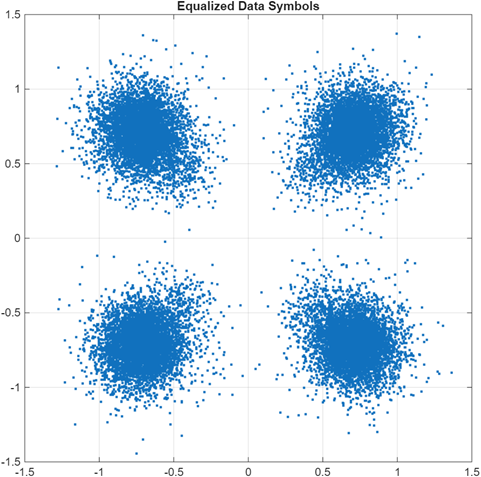
\includegraphics[width=0.3\textwidth]{figures/chap3_channel/c2_2.png} &
        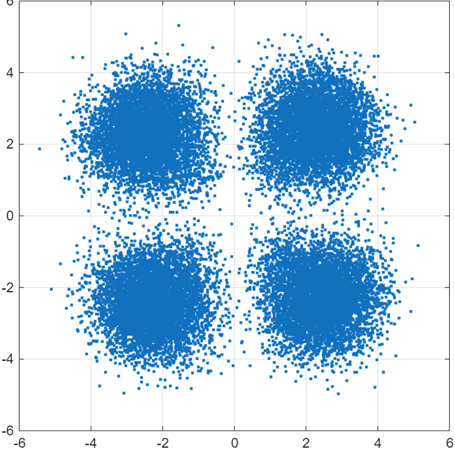
\includegraphics[width=0.3\textwidth]{figures/chap3_channel/c1_4.png} &
        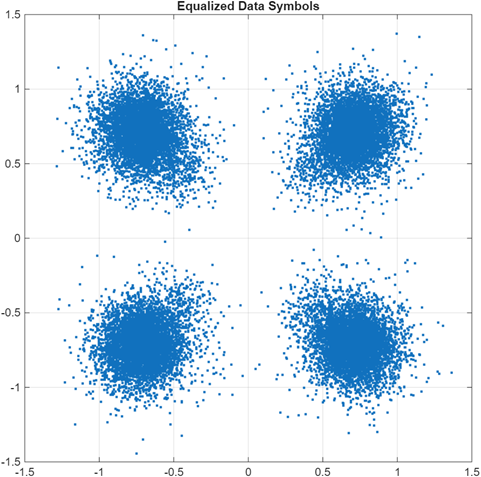
\includegraphics[width=0.3\textwidth]{figures/chap3_channel/c2_2.png} \\
        \small (a) MMSE Equalization & \small (b) LS Equalization & \small (c) No Equalization
    \end{tabular}
    \caption[Channel 2: Equalization Performance]{%
        Comparison of 4-QAM constellations for Channel 2: (a) MMSE equalization effectively minimizes clustering spread; 
        (b) LS equalization displays characteristic noise enhancement; 
        (c) Unequalized signal showing an open eye status due to low intrinsic distortion.
    }%
    \label{fig:ch2_constellations}%
\end{figure}


\begin{figure}[!ht]
    \ffigbox[\FBwidth]{%
        \begin{tabular}{cc}
            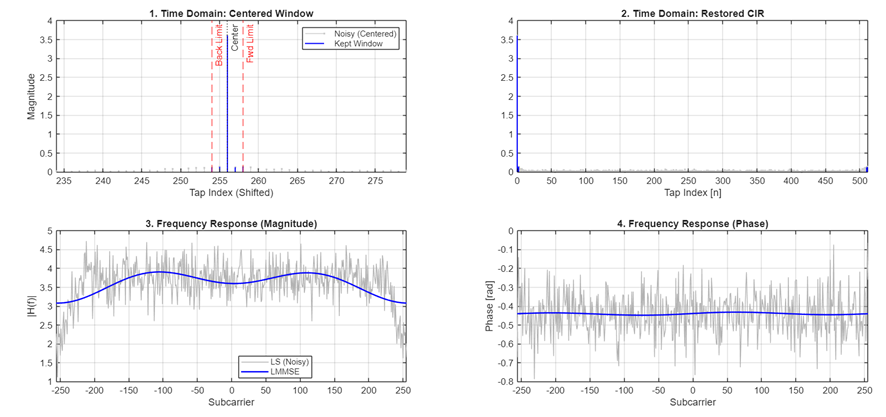
\includegraphics[width=0.67\textwidth]{figures/chap3_channel/c2_1.png} & 
            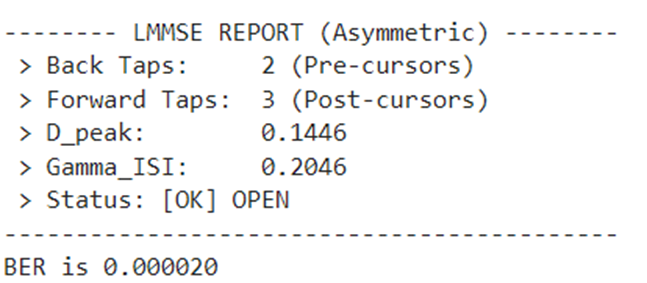
\includegraphics[width=0.27\textwidth]{figures/chap3_channel/c2_3.png} \\
        \end{tabular}
    }{%
        \caption[Channel 2: Response and ISI Report]{%
            (Left) Time domain CIR windowing and Frequency Response magnitude for Channel 2. 
            (Right) LMMSE numerical report indicating $\gamma_{\text{ISI}} = 0.2046$ with an [OK] OPEN status.
        }%
        \label{fig:ch2_report}%
    }
\end{figure}

\newpage
\section{Channel 3}
\begin{figure}[!ht]
    \centering
    \captionsetup{parskip = .5\baselineskip plus 1pt}
    \begin{tabular}{ccc}
        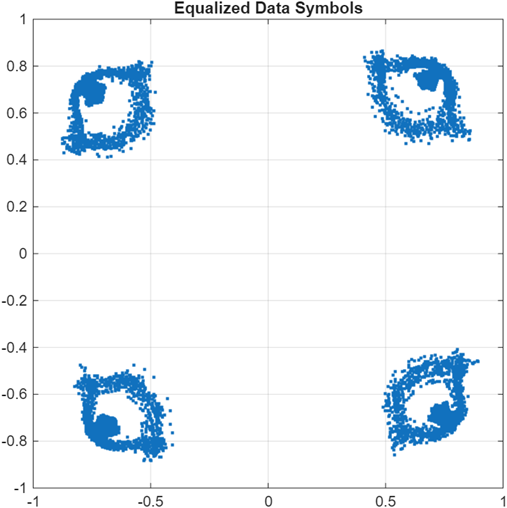
\includegraphics[width=0.3\textwidth]{figures/chap3_channel/c3_3.png} &
        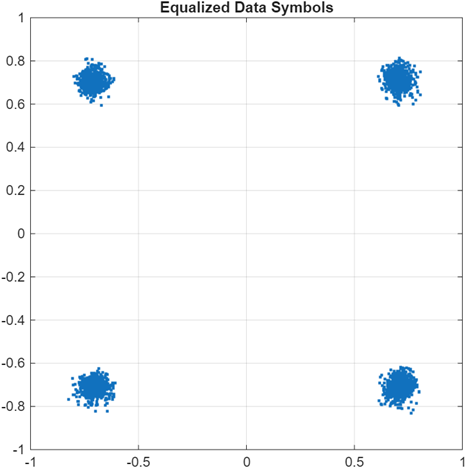
\includegraphics[width=0.3\textwidth]{figures/chap3_channel/c3_4.png} &
        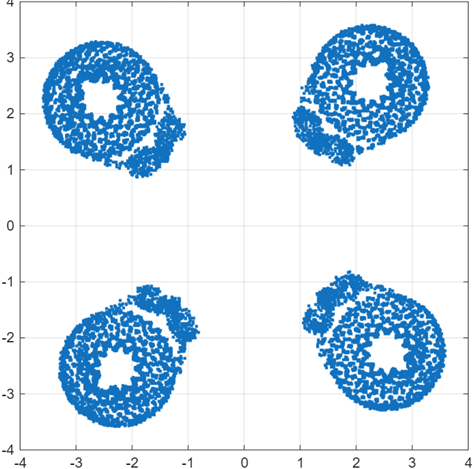
\includegraphics[width=0.3\textwidth]{figures/chap3_channel/c3_5.png} \\
        \small (a) MMSE Equalization & \small (b) LS Equalization & \small (c) No Equalization
    \end{tabular}
    \caption[Comparison of Equalization Techniques]{%
        Constellation comparison: (a) MMSE equalization provides optimal clustering; 
        (b) LS equalization shows higher noise sensitivity; 
        (c) Unequalized signal with a closed eye pattern due to severe ISI.
    }%
    \label{fig:constellation_comparison}%
\end{figure}



\begin{figure}[!ht]
    \ffigbox[\FBwidth]{%
        \begin{tabular}{cc}
            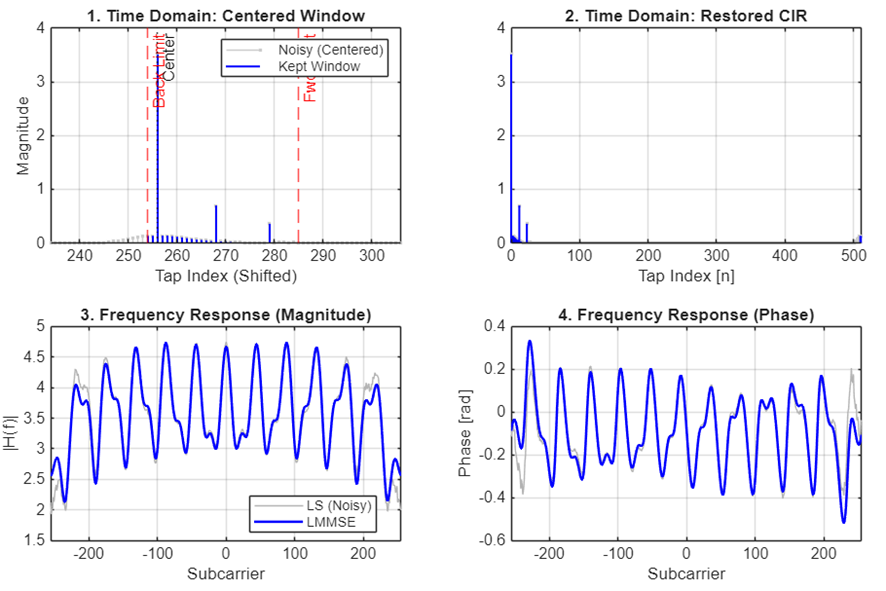
\includegraphics[width=0.67\textwidth]{figures/chap3_channel/c3_1.png} & 
            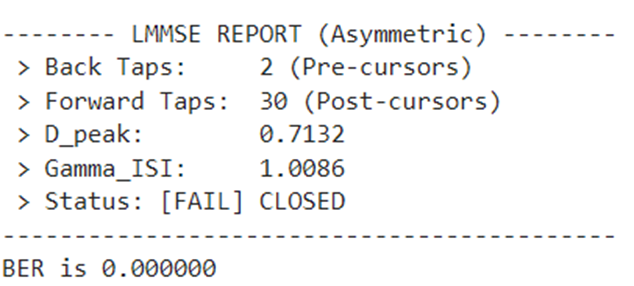
\includegraphics[width=0.27\textwidth]{figures/chap3_channel/c3_2.png} \\
        \end{tabular}
    }{%
        \caption[Channel Estimation and ISI Report]{%
            (Left) Time domain CIR windowing and Frequency Response analysis. 
            (Right) LMMSE numerical report with $\gamma_{\text{ISI}} = 1.0086$, confirming a closed eye status.
        }%
        \label{fig:channel_estimation_summary}%
    }
\end{figure}



\begin{figure}[!ht]
    \fcapside[\FBwidth]{%
        \captionsetup{parskip = .5\baselineskip plus 1pt}%
        \caption[]{%
            Channel Power Delay Profile (PDP).
        }%
        \label{fig:isi-dispersion}%
    }{%
        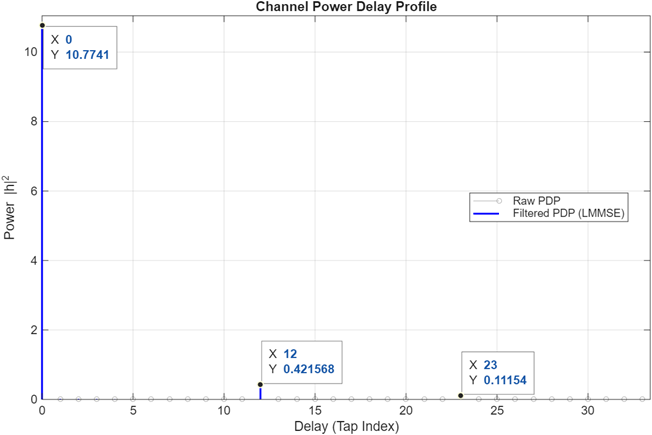
\includegraphics[width=0.60\textwidth]{figures/chap3_channel/c3_6.png}
    }
\end{figure}


\newpage
\section{Channel 4}
\begin{figure}[!ht]
    \centering
    \captionsetup{parskip = .5\baselineskip plus 1pt}
    \begin{tabular}{cc}
        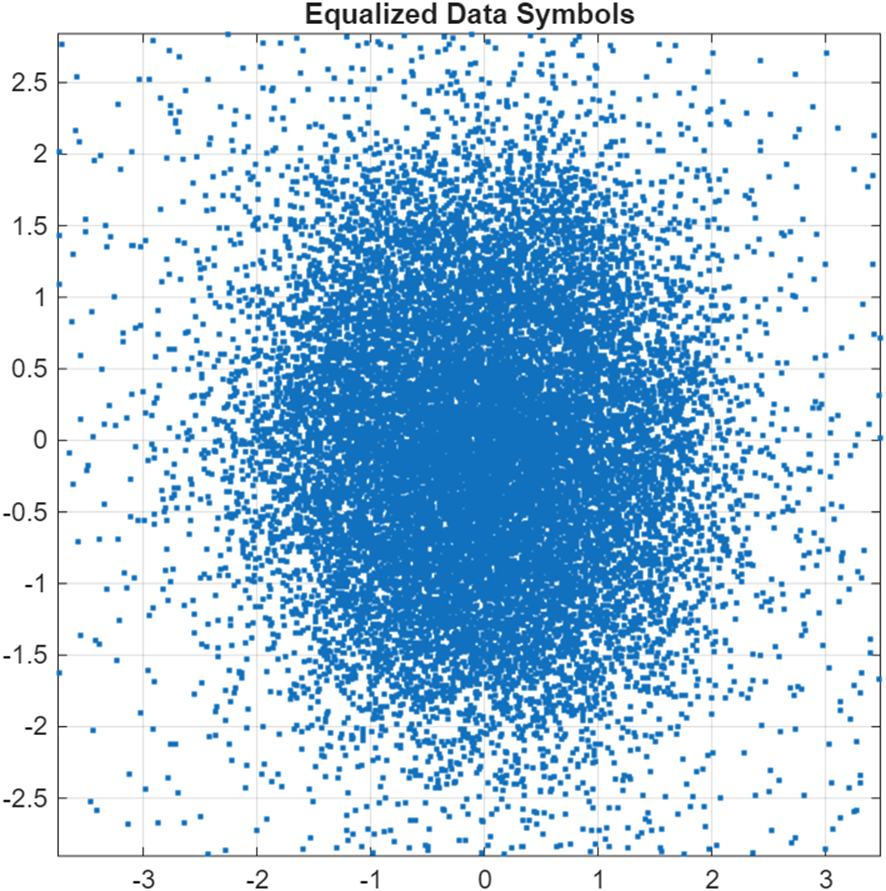
\includegraphics[width=0.45\textwidth]{figures/chap3_channel/c4_1.png} &
        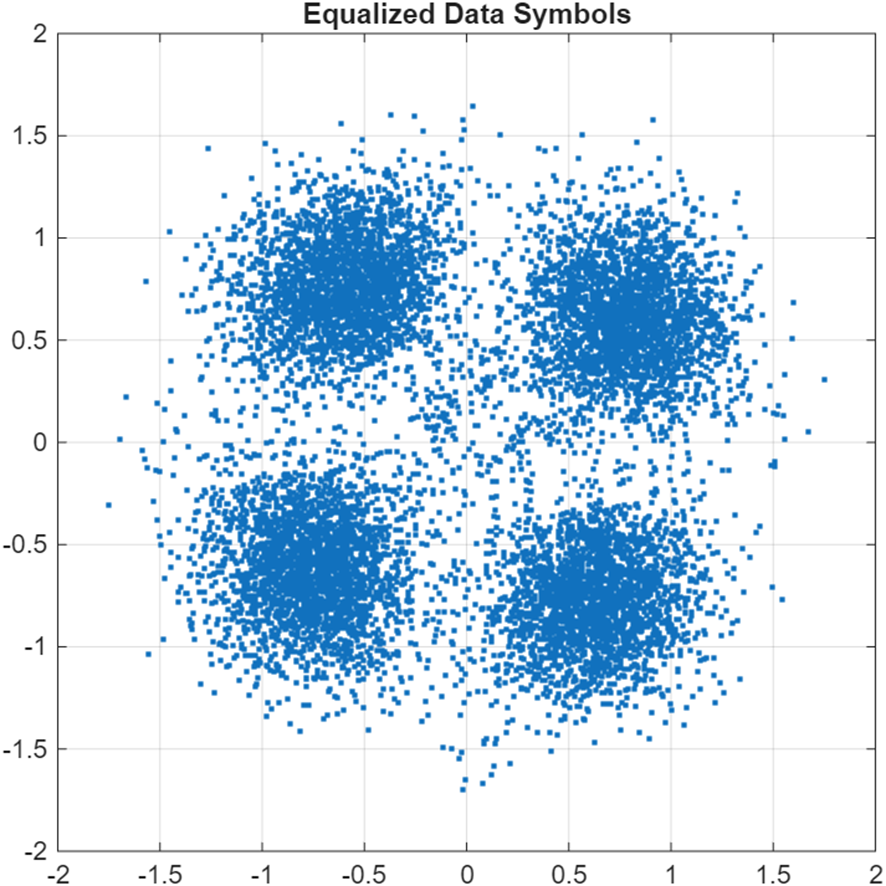
\includegraphics[width=0.45\textwidth]{figures/chap3_channel/c4_3.png} \\
        \small (a) Initial Equalized Symbols & \small (b) Improved Sideband Reception
    \end{tabular}
    \caption[Channel 4: Band-Rejection Equalization Comparison]{%
        Comparison of received 4-QAM constellations for Channel 4: (a) High BER reception due to band-rejection characteristics; 
        (b) Improved constellation achieved by activating sideband subcarriers, leading to lower bit error rates.
    }%
    \label{fig:ch4_constellations}%
\end{figure}


\begin{figure}[!ht]
    \ffigbox[\FBwidth]{%
        \begin{tabular}{cc}
            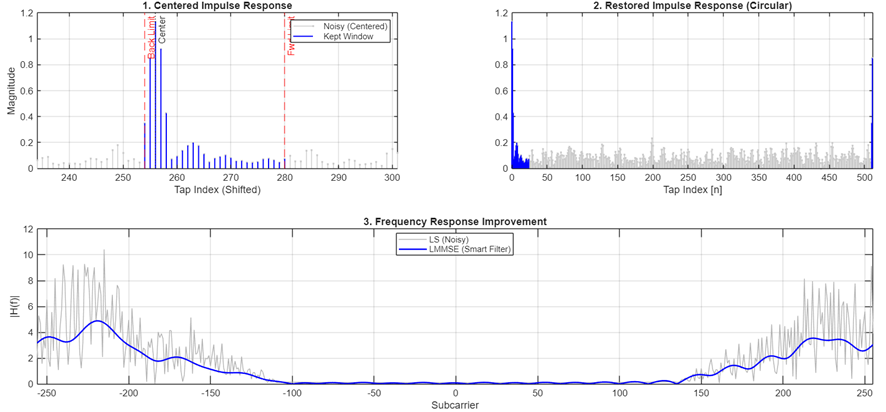
\includegraphics[width=0.67\textwidth]{figures/chap3_channel/c4_6.png} & 
            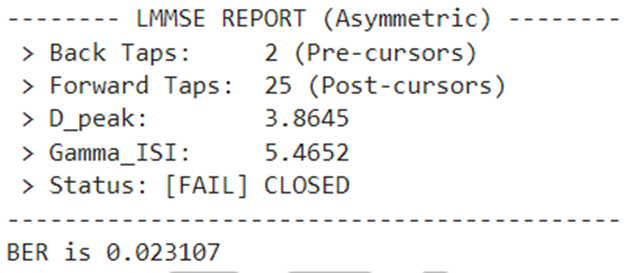
\includegraphics[width=0.27\textwidth]{figures/chap3_channel/c4_4.png} \\
        \end{tabular}
    }{%
        \caption[Channel 4: Frequency Response and Improved Report]{%
            (Left) Frequency response analysis revealing a significant band-rejection notch in the central subcarriers. 
            (Right) Improved LMMSE report for sideband transmission, showing an optimized status despite a high $\gamma_{\text{ISI}} = 5.4652$.
        }%
        \label{fig:ch4_frequency_report}%
    }
\end{figure}


\begin{figure}[!ht]
    \fcapside[\FBwidth]{%
        \captionsetup{parskip = .5\baselineskip plus 1pt}%
        \caption[]{%
            Signal magnitude and normalized correlation metric for Channel 4 frame detection.
        }%
        \label{fig:ch4_correlation}%
    }{%
        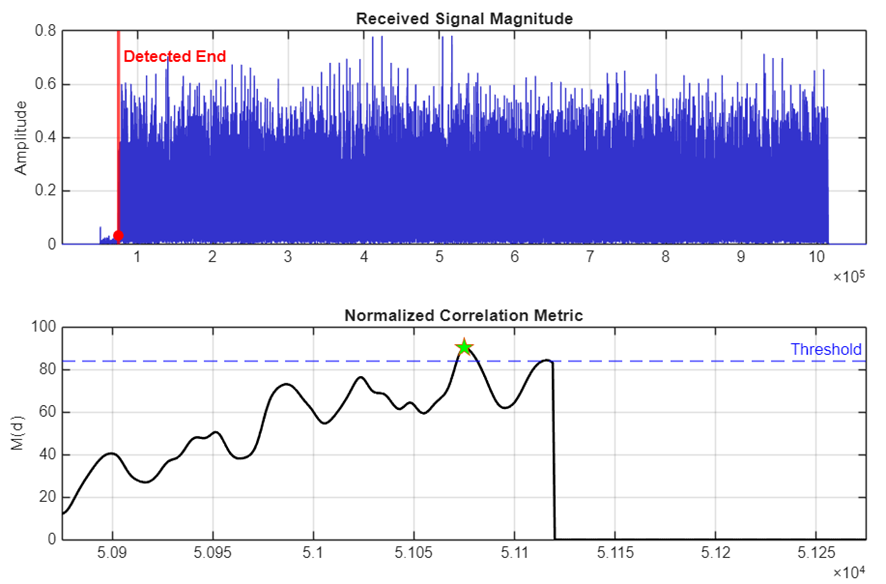
\includegraphics[width=0.60\textwidth]{figures/chap3_channel/c4_5.png}
    }
\end{figure}



\newpage
\section{Channel 5}

\begin{figure}[!ht]
    \fcapside[\FBwidth]{%
        \captionsetup{parskip = .5\baselineskip plus 1pt}%
        \caption[Channel 5: MMSE Equalized Symbols]{%
            Recovered 4-QAM constellation for Channel 5 utilizing LMMSE equalization to mitigate severe ISI.
        }%
        \label{fig:ch5_constellation}%
    }{%
        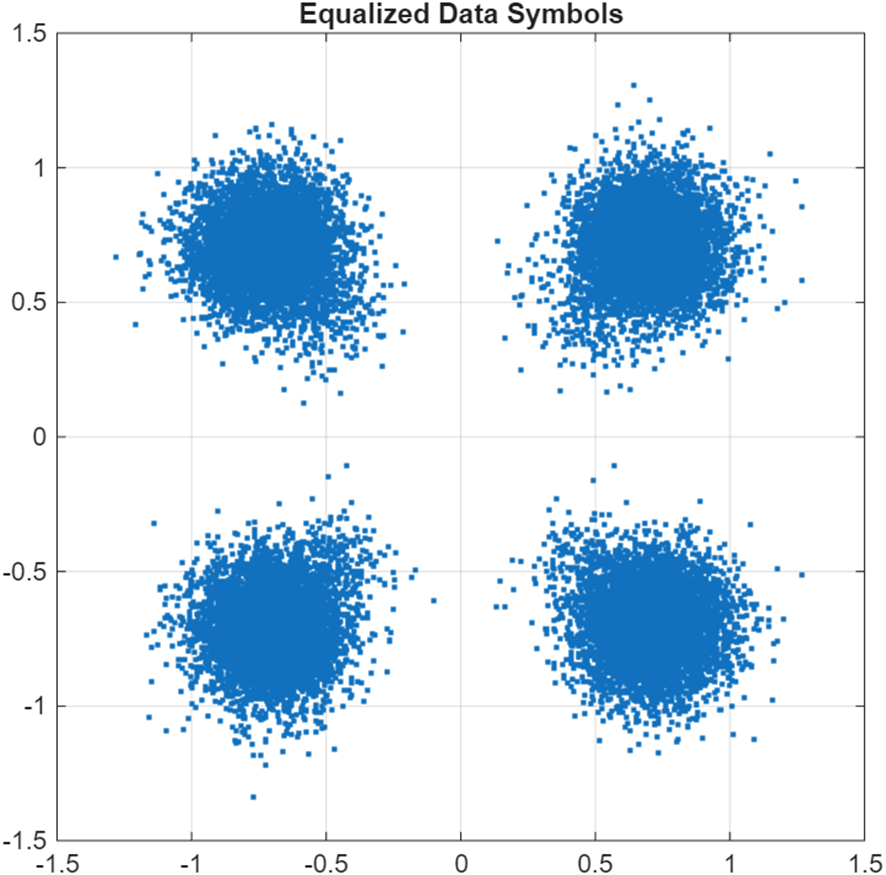
\includegraphics[width=0.60\textwidth]{figures/chap3_channel/c5_1.png}
    }
\end{figure}

\begin{figure}[!ht]
    \centering
    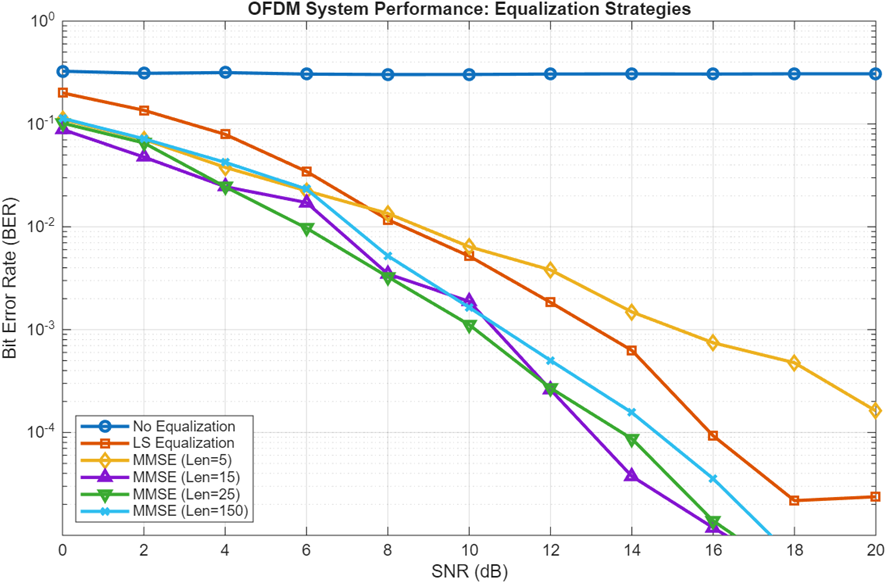
\includegraphics[width=0.85\textwidth]{figures/chap3_channel/c5_2.png}
    \caption[Channel 5: BER Performance Comparison]{%
        Bit Error Rate (BER) performance curves for Channel 5. The plot compares the performance of an unequalized system, LS equalization, and MMSE equalization with varying filter lengths ($L=5, 15, 25, 150$).
    }%
    \label{fig:ch5_ber_performance}%
\end{figure}

\begin{figure}[!ht]
    \ffigbox[\FBwidth]{%
        \begin{tabular}{cc}
            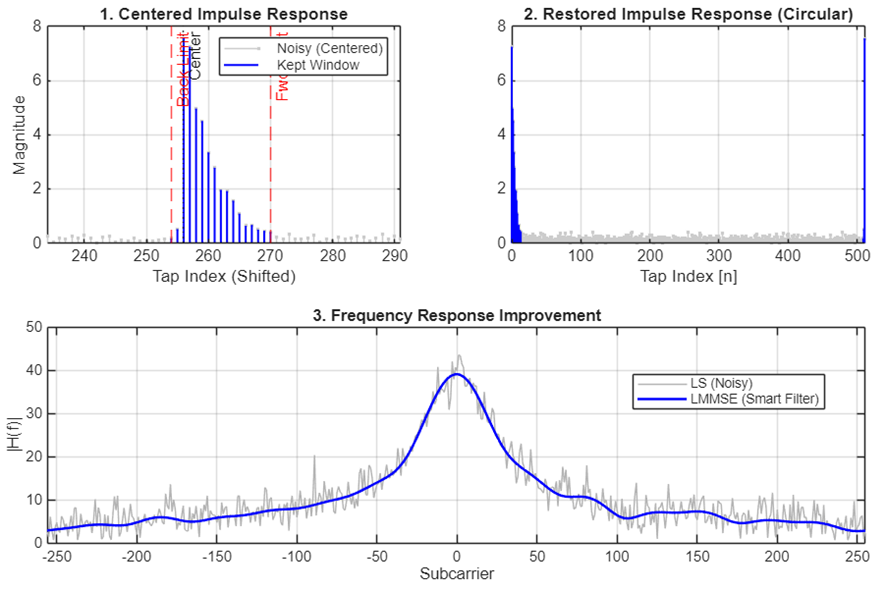
\includegraphics[width=0.67\textwidth]{figures/chap3_channel/c5_3.png} & 
            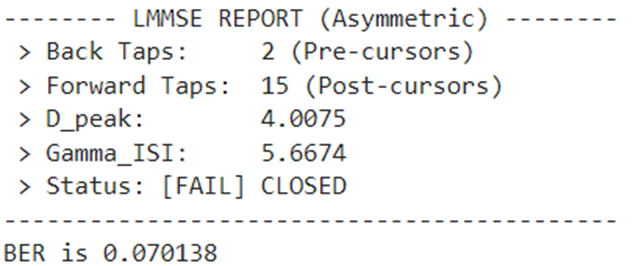
\includegraphics[width=0.27\textwidth]{figures/chap3_channel/c5_4.png} \\
        \end{tabular}
    }{%
        \caption[Channel 5: Estimation and Numerical Report]{%
            (Left) Time-domain CIR and Frequency Response improvement analysis. 
            (Right) LMMSE numerical report showing the critical ISI level $\gamma_{\text{ISI}} = 5.6674$ and a [FAIL] CLOSED status.
        }%
        \label{fig:ch5_numerical_summary}%
    }
\end{figure}

\begin{figure}[!ht]
    \fcapside[\FBwidth]{%
        \captionsetup{parskip = .5\baselineskip plus 1pt}%
        \caption[]{%
            Channel 5 Power Delay Profile (PDP) comparing raw energy and filtered LMMSE distribution.
        }%
        \label{fig:ch5_pdp_analysis}%
    }{%
        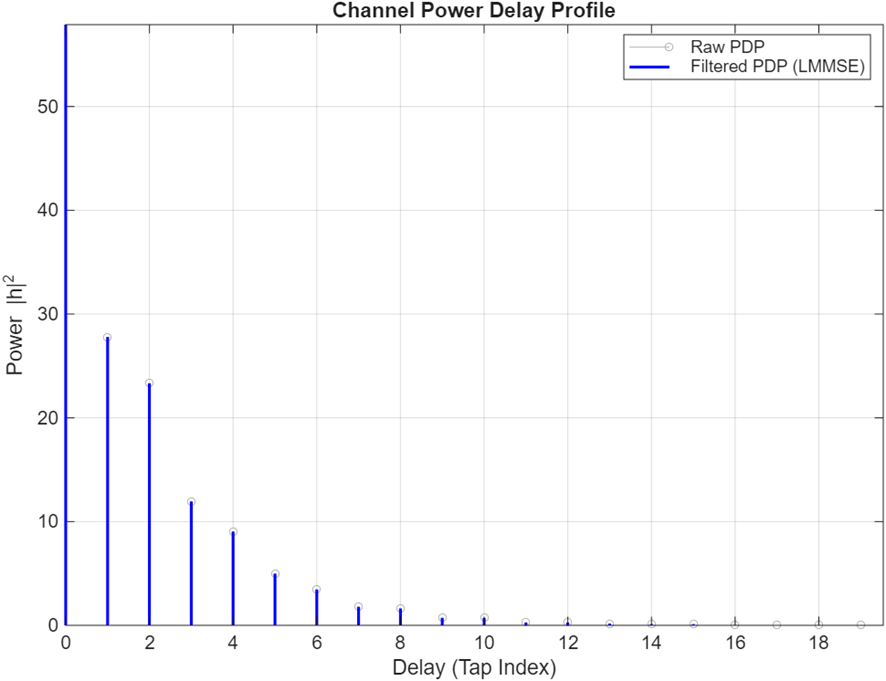
\includegraphics[width=0.60\textwidth]{figures/chap3_channel/c5_5.png}
    }
\end{figure}


%%%%%%%%%%%%%%%%%%%%%%%%%%%%%%%%%%%%%%%%%%%%%%%%%%%%%%%%%%%%%%%
%%%%%%%%%%%%%%%%%%%%%%%%%%%%%%%%%%%%%%%%%%%%%%%%%%%%%%%%%%%%%%%
%%%%%%%%%%%%%%%%%%%%%%%%%%%%%%%%%%%%%%%%%%%%%%%%%%%%%%%%%%%%%%%

\newpage
\section{Transmission Experiments} \label{sec:appendix_transmission}

\begin{figure}[!ht]
    \centering
    \captionsetup{parskip = .5\baselineskip plus 1pt}
    \begin{tabular}{cc}
        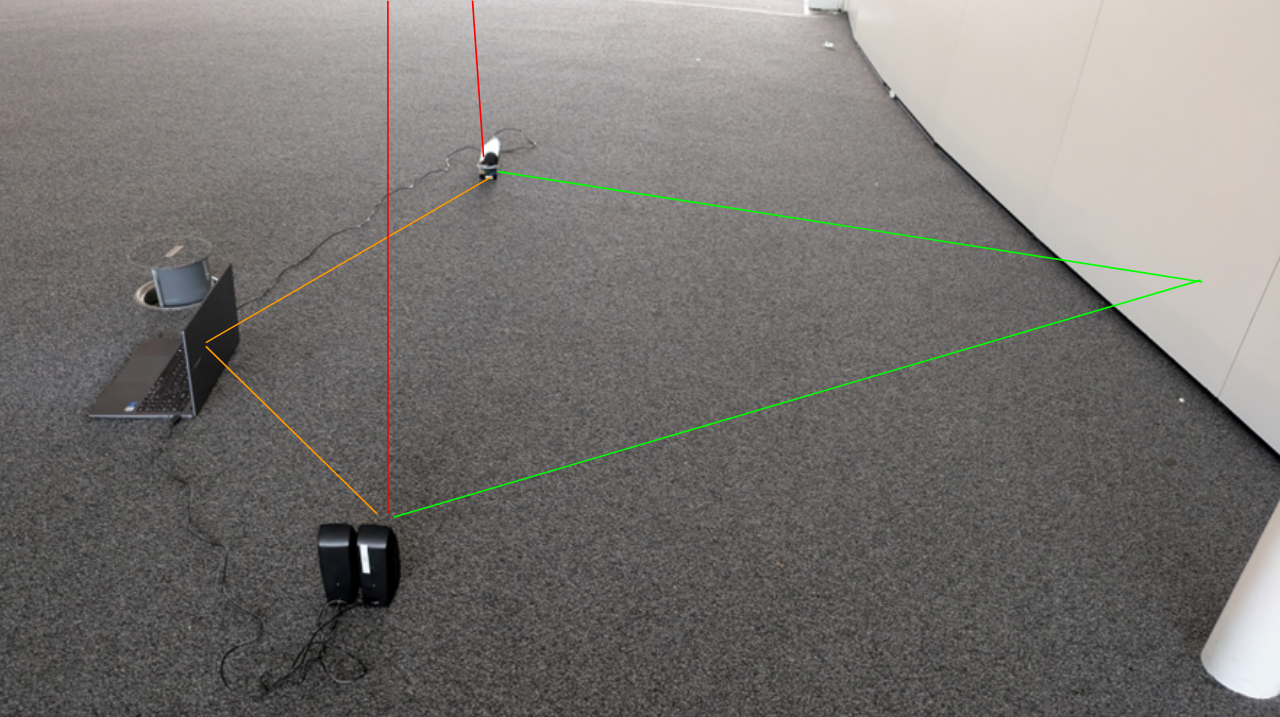
\includegraphics[width=0.47\textwidth]{figures/chap5_transmission/imag1.png} &
        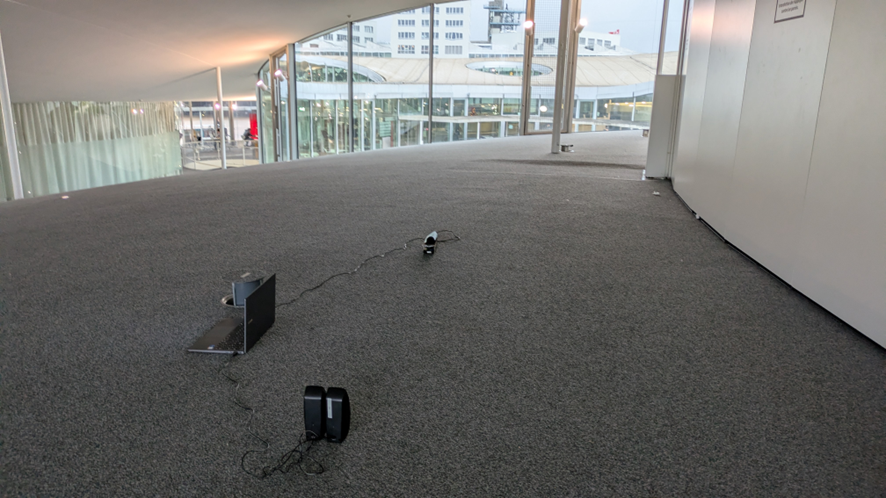
\includegraphics[width=0.47\textwidth]{figures/chap5_transmission/imag2.png} \\
        \small (a) Tx/Rx Setup & \small (b) Environment View
    \end{tabular}
    \caption[Experimental Setup]{%
        Physical experimental setup showing the acoustic transmission environment.
        (a) Relative positioning of the laptop (transmitter/receiver processing) and speakers.
        (b) Wide view of the room characterized by carpeted flooring and glass walls.
    }%
    \label{fig:trans_setup}%
\end{figure}

\begin{figure}[!ht]
    \ffigbox[\FBwidth]{%
        \begin{tabular}{cc}
            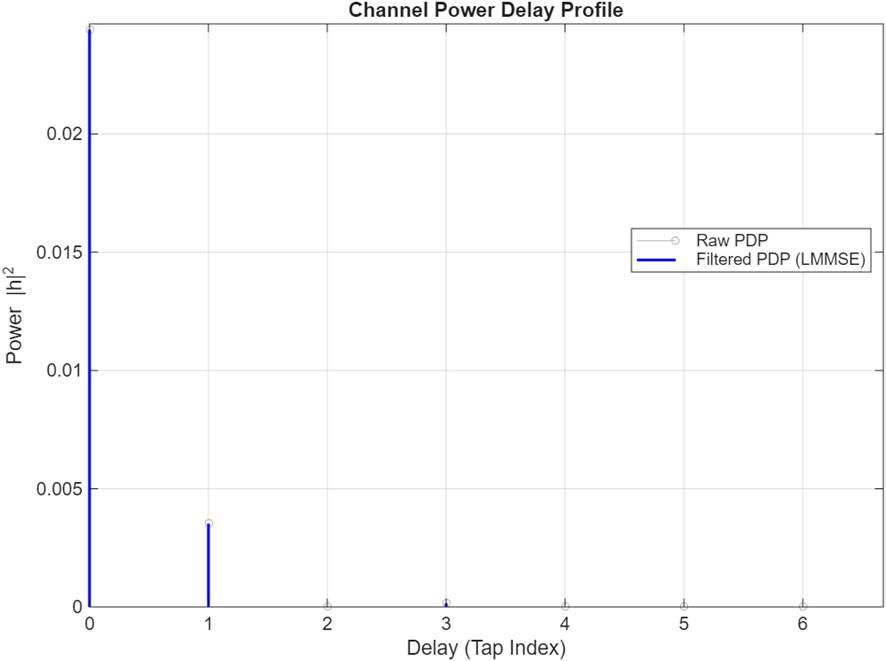
\includegraphics[width=0.48\textwidth]{figures/chap5_transmission/imag6.png} & 
            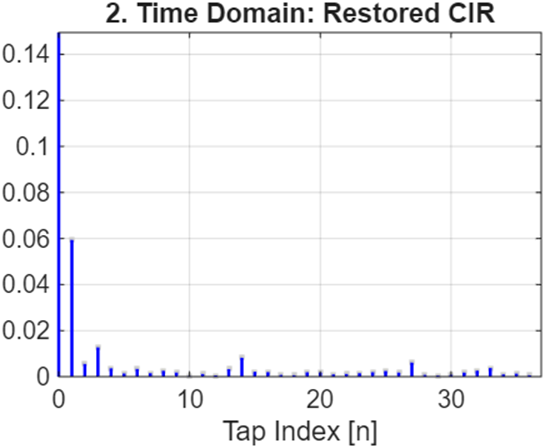
\includegraphics[width=0.45\textwidth]{figures/chap5_transmission/imag7.png} \\
        \end{tabular}
    }{%
        \caption[Channel Impulse Analysis]{%
            (Left) Channel Power Delay Profile (PDP) showing the main path and multipath components. 
            (Right) Restored Time Domain Channel Impulse Response (CIR) used for equalization.
        }%
        \label{fig:trans_cir_pdp}%
    }
\end{figure}

\begin{figure}[!ht]
    \ffigbox[\FBwidth]{%
        \begin{tabular}{cc}
            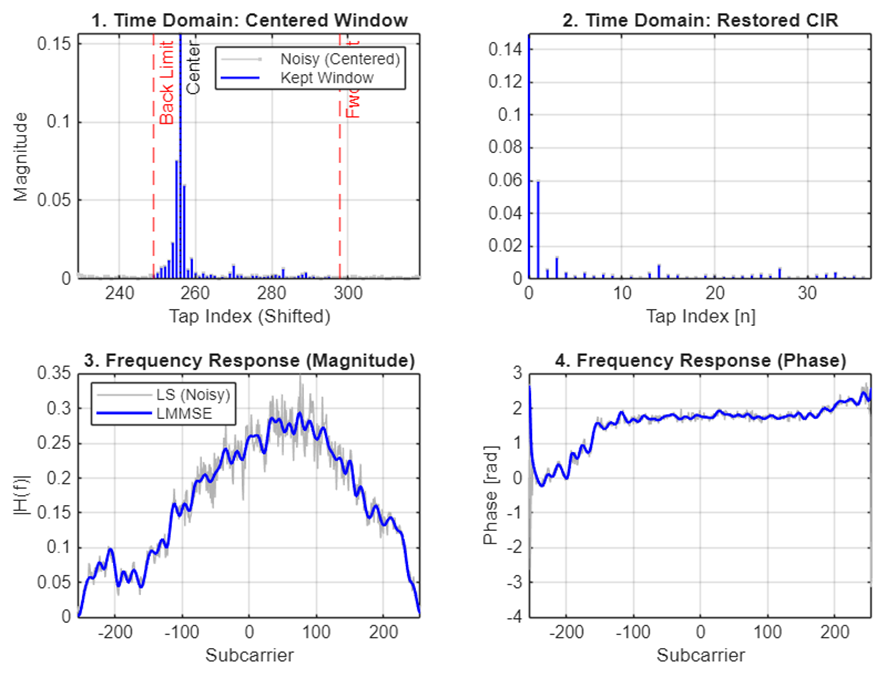
\includegraphics[width=0.64\textwidth]{figures/chap5_transmission/imag4.png} & 
            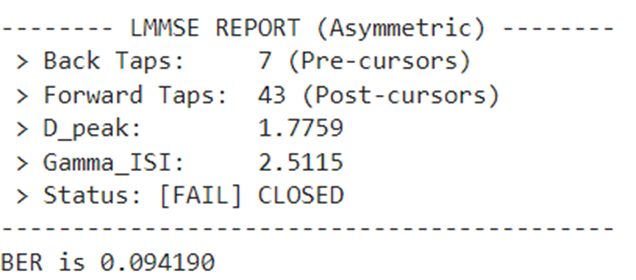
\includegraphics[width=0.29\textwidth]{figures/chap5_transmission/imag8.png} \\
        \end{tabular}
    }{%
        \caption[LMMSE Estimation Report]{%
            (Left) Detailed channel estimation plots: windowing strategy, CIR, and frequency response (magnitude and phase). 
            (Right) LMMSE numerical report showing estimation parameters, $\gamma_{\text{ISI}} = 2.5115$, and a resulting BER of \num{0.094190}.
        }%
        \label{fig:trans_lmmse_report}%
    }
\end{figure}

\begin{figure}[!ht]
    \fcapside[\FBwidth]{%
        \captionsetup{parskip = .5\baselineskip plus 1pt}%
        \caption[Image Transmission Result]{%
            Visual comparison between the original transmitted test pattern and the received image after equalization and decoding, illustrating the impact of the acoustic channel.
        }%
        \label{fig:trans_image_result}%
    }{%
        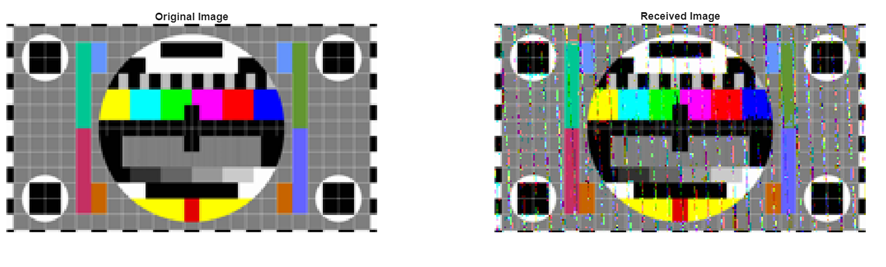
\includegraphics[width=0.75\textwidth]{figures/chap5_transmission/imag5.png}
    }
\end{figure}

\references

\end{document}
